\chapter{Humanoid motion generation in a world of stairs}
\label{ch:humanoid-motion-generation-WoS}

% Define and set new counter for environment procedure:
\newcounter{procedure}
\makeatletter
\AtBeginEnvironment{procedure}{\let\c@algocf\c@procedure}
\makeatother

\renewcommand\textfraction{0.0}
\renewcommand\bottomfraction{1.0}
\renewcommand\topfraction{1.0}
\renewcommand\dbltopfraction{1.0}
\setcounter{topnumber}{8}
\setcounter{dbltopnumber}{8}
\setcounter{bottomnumber}{8}
\setcounter{totalnumber}{8}
	
	%%%%%%%%%%%%%%%%%%%%%%%%
	%%%%% ABSTRACT %%%%%%%%%
	%%%%%%%%%%%%%%%%%%%%%%%%
	
%\begin{abstract} 
%Consider the problem of generating humanoid motions in an environment consisting of horizontal patches located at different heights ({\em world of stairs}).
%To this end, the chapter proposes an integrated scheme which combines footstep planning and gait generation. 
%In particular, footsteps are produced by a randomized algorithm that guarantees both feasibility and quality of the plan according to a chosen criterion; whereas for 3D gait generation we devise an ad hoc extension of the Intrinsically Stable MPC scheme. 
%In its basic form, the proposed scheme addresses the off-line case (known environments), but a sensor-based adaptation is developed for the on-line case (unknown environments) based on an anytime version of the footstep planner.
%In order to validate the proposed approach, we present simulations in CoppeliaSim for the HRP-4 humanoid robot navigating scenarios of different complexity, both in the on-line and off-line case.
%\end{abstract}

In this chapter we consider the problem of generating a humanoid motion in a
\textit{world of stairs}, a specific kind of uneven ground consisting of
horizontal patches located at different heights. In order to successfully
achieve this, it is necessary to plan a footstep sequence and a whole body
motion for the humanoid realizing such sequence. We choose to approach the
problem by keeping these two stages separate. The reason for this choice is
that in this way we can better control the quality of the produced motions.
In fact, the quality of the footstep plan can be evaluated based on global
requirements, such as the number of steps taken, or a different performance
index. As for the quality of the motion itself, this should be mainly addressed
by its capability to satisfy all the required constraints, in order to avoid
falls and instabilities. Maintaining a separation between planning and control
also greatly simplifies the tuning because the domain in which any given
parameter has effect is reduced.

Keeping planning and control separated is relatively straightforward when the
planning is done off-line. However, it might be more difficult to realize if
one wants to allow for on-line planning and replanning. In this chapter,
we will discuss an on-line architecture that achieves this by having short
planning stages interleaved with the motion, in such a way that the planning
can fully utilize sensor information gathered by the robot as it moves, and
that the robot itself can take advantage of the on-line planner to find more
efficient and safe footstep sequences.
Moreover, we consider planning both in off-line situations, in which the
environment is completely known, and on-line situations, in which the geometry
of the environment is not known in advance and must be reconstructed by the
robot itself during motion using on-board sensors. In this case, planning and
execution are interdependent: the former clearly requires the latter in order
to determine where to place the footsteps, but the converse is also true, as the
real-time motion of the robot is necessary to acquire information about the
environment.
	
\section{Problem formulation}
\label{sec:WoS:Formulation}
In the situation of interest (Fig.~\ref{fig:WoS:WoSScenario}), a humanoid robot
moves in a {\em world of stairs}, a specific kind of uneven ground consisting of
horizontal patches that {\em (i)} are located at different heights, and
{\em (ii)} constitute a partition\footnote{This implies that the whole
volume of space below any horizontal patch is occupied.} of $\RealSet^2$. 
Depending on its elevation with respect to the neighboring areas, a patch may
be accessible for the humanoid to climb on from an appropriate direction;
otherwise, it actually represents an {\em obstacle} to be avoided.
Any accessible patch may be stepped on, stepped over or even circumvented,
depending on the generated motion.  

\begin{figure}
    \centering
    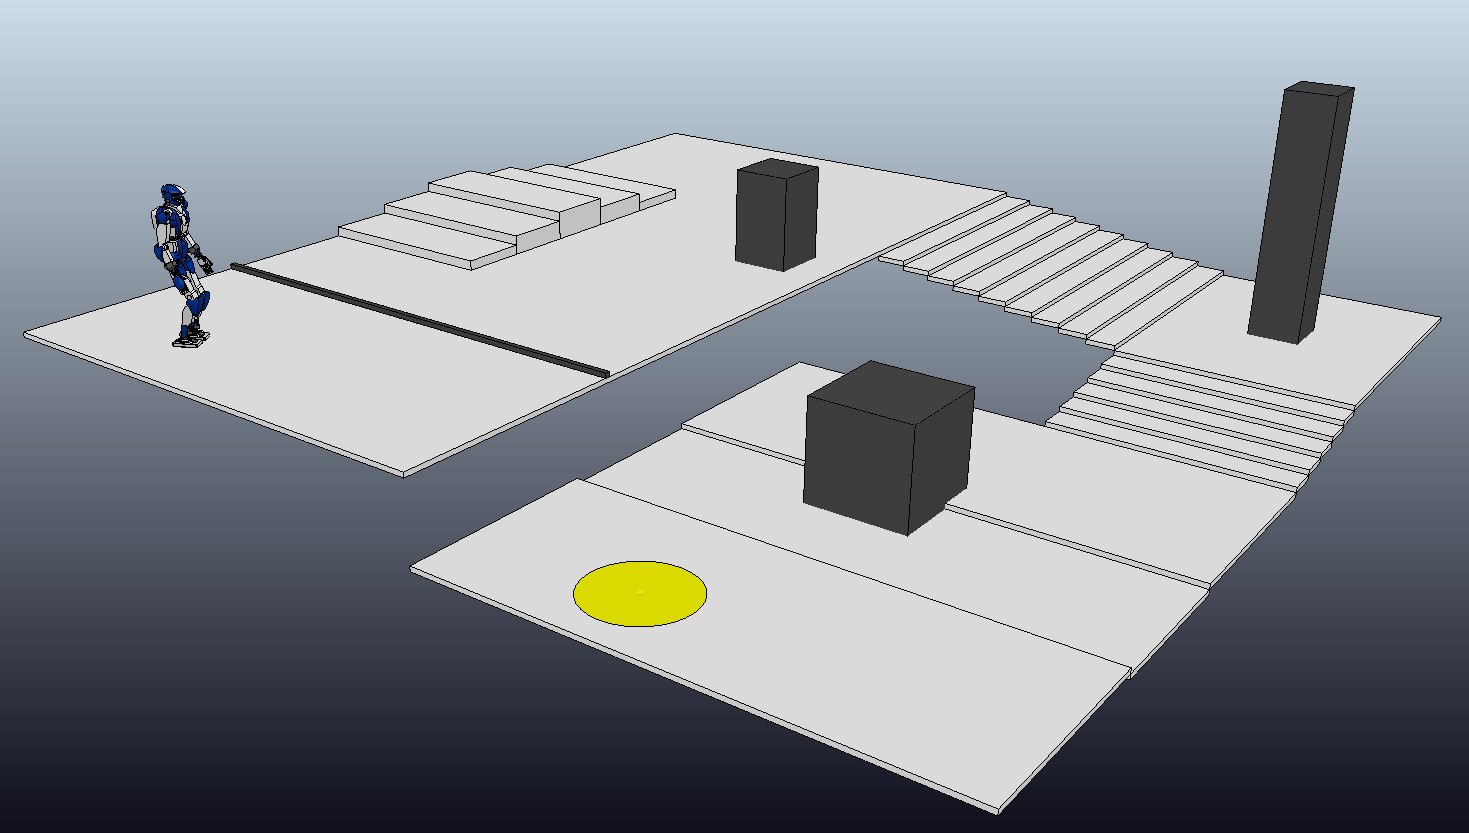
\includegraphics[width=0.9\textwidth]{figures/WoS_Scenario.jpeg}
    \caption{An instance of the considered problem. The robot must reach the
        goal region (in yellow) by traversing a {\em world of stairs}.
        Patches that are not visible correspond to infinitely deep holes or
        trenches.}
    \label{fig:WoS:WoSScenario}
\end{figure}

The mission of the robot is to reach a certain goal region $\cal G$, which will
belong in general to a single patch (Fig.~\ref{fig:WoS:WoSScenario}).
In particular, this locomotion task is accomplished as soon as the robot
places a footstep inside $\cal G$.

We want to devise a complete framework enabling the humanoid to plan and
execute a motion to fulfill the assigned task in the world of stairs.
This requires addressing two fundamental problems: finding a 3D footstep plan
and generating a variable-height gait that is consistent with such plan.
Footstep planning consists in finding both footstep placements and swing foot
trajectories between them; overall, the footstep plan must be feasible
(in a sense to be formally defined later) for the humanoid, given the
characteristics of the environment. Gait generation consists in finding a
CoM trajectory which realizes the footstep plan while guaranteeing dynamic
balance of the robot at all time instants. From the trajectories of the CoM
and the feet, a whole-body motion may be computed using inverse kinematics
methods.

In particular, we will address two versions of the above problem, henceforth
referred to as the \textit{off-line} and \textit{on-line} case. In the first,
the geometry of the environment is completely known in advance, while in the
second it is reconstructed by the robot itself as it moves. 
In the following we describe the architectures designed for the off-line
and on-line case supposing that the environment is static.
However, we will also show that the latter can be used effectively in
dynamic environments, thanks to its fast replanning capabilities. 

The problem will be solved under the following assumptions.

\begin{itemize}

\item[A1] Information about the environment is maintained in an
{\em elevation map} ${\cal M}_{z}$, i.e., a 2.5D grid map of equally-sized
cells that, whenever needed, can be queried as $z = {\cal M}_{z}(x,y)$, to
provide the height of the ground at the cell having coordinates $(x,y)$
\cite{Burgard2016WorldModeling}.
In the off-line case, ${\cal M}_{z}$ is available a priori, while in the
on-line case it must be incrementally built by the humanoid based on sensory
information. 
    
\item[A2] The humanoid is equipped with a head-mounted RGB-D camera, which is
used for localization in both the off-line and on-line cases, and also updating
the elevation map ${\cal M}_{z}$ in the latter.
    
\item[A3] The humanoid is endowed with a localization module which provides an
estimate of the camera pose at each time instant, based on information gathered
by the RGB-D camera. This is used in both the off-line and on-line cases.

\item[A4] The friction between the robot feet and the ground is sufficiently
large to avoid slipping at the contact surfaces\footnote{Since our objective
is to generate walking gaits in a world of stairs, we expect that the horizontal
components of the ground reaction forces will be rather limited with respect
to the vertical components, making this assumption reasonable. Nevertheless,
the constraint that ground reaction forces must always be contained in the
friction cone can be incorporated in our formulation; this extension would be
required in the case of non-horizontal contact surfaces.}.

\end{itemize}

In the off-line case, a complete footstep plan leading to the goal region
$\cal G$ will be computed before the humanoid starts to move. In the
on-line case, the footstep plan will instead be updated during motion, based on
new information added to ${\cal M}_{z}$. 

In the following, we first address in full detail the off-line case and then
proceed to extending the proposed approach to the on-line case.

\section{The off-line case} 
\label{sec:WoS:offlineCase}
We start this section by describing the general structure of the proposed
method. Then we will describe the footsep planner and present some simulations.
The gait generation scheme used is the one presented in Chapter \ref{ch:ISMPC}.

\subsection{General architecture}
\label{sec:WoS:offlineCase:GeneralArchitecture}
To solve the described problem in the off-line case, we adopt the architecture
shown in Fig.~\ref{fig:WoS:blockScheme1}, in which the main components are the
footstep planning, gait generation and localization modules.

\begin{figure}
    \centering
    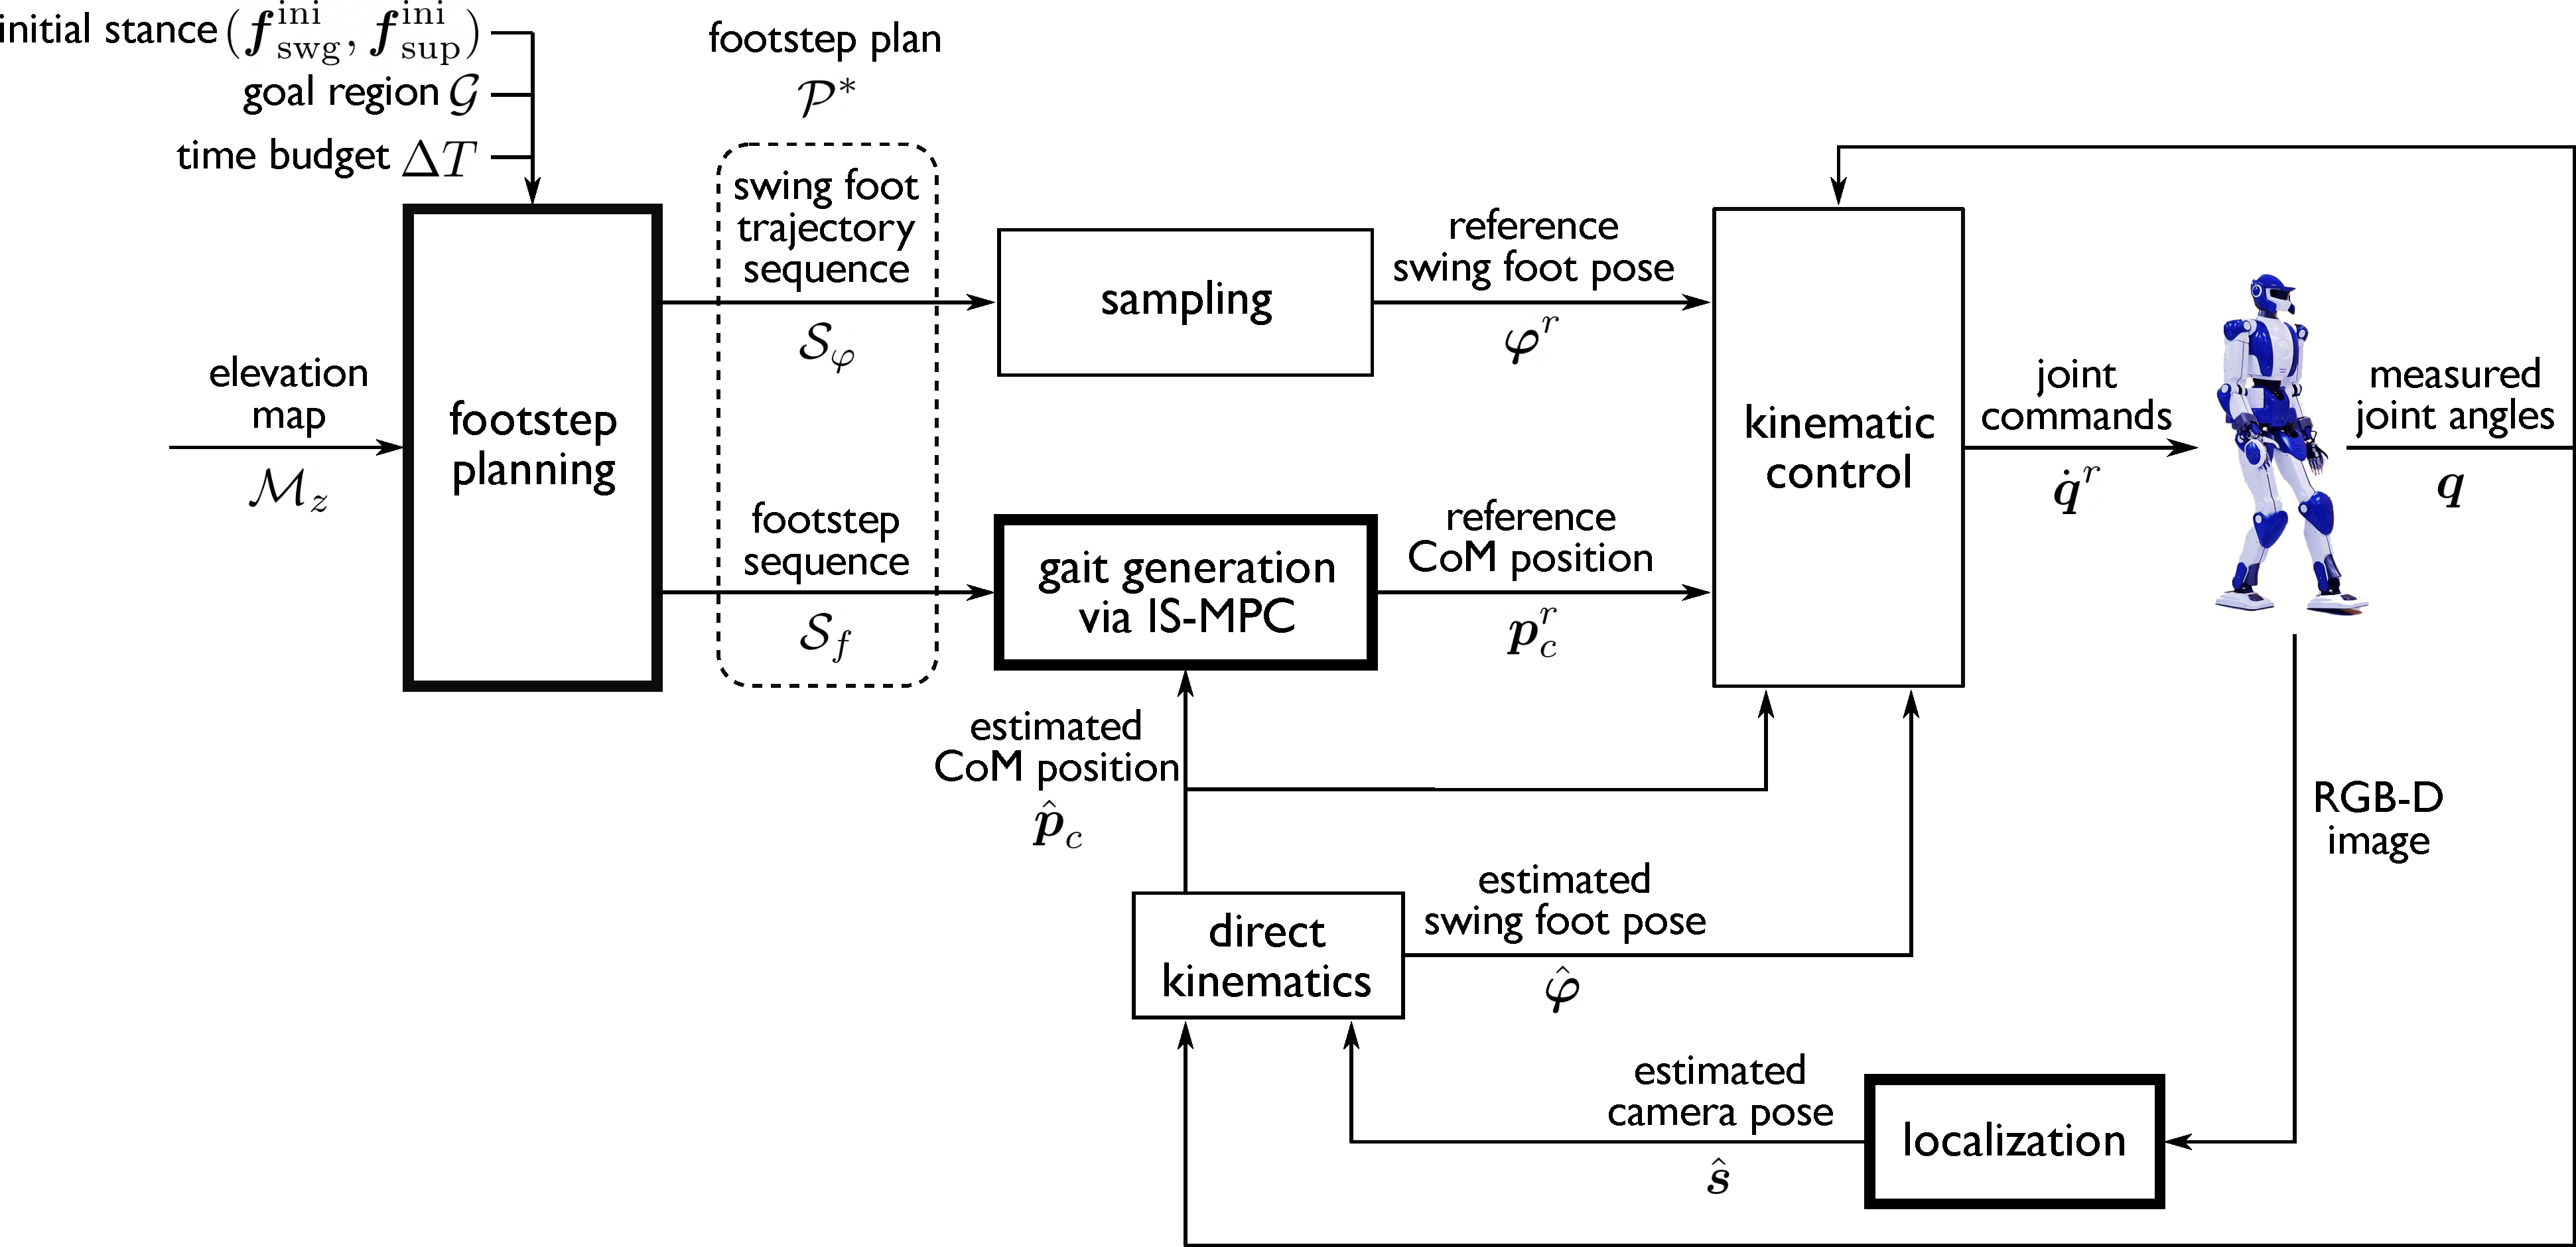
\includegraphics[width=\textwidth]{figures/BlockSchemeOffline.pdf}
    \caption{Block scheme of the proposed solution approach for the off-line case.}
    \label{fig:WoS:blockScheme1}
\end{figure}

In the following, we denote by $\bff = (x_{f}, y_{f}, z_{f}, \theta_{f})$ the
{\em pose} of a certain footstep, with $x_{f}$, $y_{f}$, $z_{f}$ representing
the coordinates of a representative point, henceforth collectively denoted as
$\bfp_f$, and $\theta_{f}$ its orientation\footnote{To represent the footstep
orientation we only use the yaw angle, as roll and pitch are always zero thanks
to the piecewise-horizontal ground assumption.}.
Moreover, a pair $(\bff_{\rm swg}, \bff_{\rm sup})$ defines a {\em stance},
i.e., the feet poses during a double support phase after which a step is
performed by moving the swing foot from $\bff_{\rm swg}$ while keeping the
support foot at $\bff_{\rm sup}$. 

The footstep planner receives in input the initial humanoid
stance\footnote{The initial support foot can be chosen arbitrarily.}
$(\bff_{\rm swg}^{\rm ini}, \bff_{\rm sup}^{\rm ini})$ at $t=0$, the goal
region $\cal G$, a time budget $\Delta T$, and the elevation map ${\cal M}_z$
representing the environment.

The time budget represents the time given to the planner to find a solution.
When this time runs over, the algorithm either returns a solution or ends
with a failure. Explicitly specifying this time as input to the algorithm
allows us to evaluate the performance of the planning module, but also proves
to be useful for the extension to the on-line case, where the time budget is
set equal to the duration of a step in order to meet the real-time requirement.

The planner works off-line to find, within $\Delta T$, an optimal
\textit{footstep plan} ${\cal P}^\ast = \{ {\cal S}_f, {\cal S}_\varphi \}$
leading to the desired goal region $\cal G$. In ${\cal P}^*$, we denote by
\begin{equation*}
    {\cal S}_f = \{\bff^1, \dots, \bff^n\}
\end{equation*}
the sequence of footstep placements, whose generic element $\bff^j$ is the
pose of the $j$-th footstep, with $\bff^1 = \bff_{\rm swg}^{\rm ini}$ and
$\bff^2 = \bff_{\rm sup}^{\rm ini}$. Also, we denote by
\begin{equation*}
    {\cal S}_\varphi = \{\bfvarphi^1, \dots, \bfvarphi^{n-2}\}
\end{equation*} 
the sequence of associated swing foot trajectories, whose generic element
$\bfvarphi^j$ is the $j$-th {\em step}, i.e., the trajectory leading the foot
from $\bff^{j}$ to $\bff^{j+2}$. Its duration $T_s^j$ is split in $T_{\rm ss}^j$
and $T_{\rm ds}^j$, respectively the single and double support phases. 
The timestamp of a generic footstep indicates the beginning of the $j$-th step,
i.e., of the $j$-th single support phase; thus, $\bff^{j}$ has an associated
timestamp $t_s^{j} = t_s^{j-1} + T_s^{j-1}$, with $t_s^{1}=0$.

Once the footstep plan has been generated, the sequence of footsteps
${\cal S}_{f}$ is sent to a gait generator based on IS-MPC
(Chapter \ref{ch:ISMPC}), which computes in real time a variable-height
CoM trajectory that
is compatible with ${\cal S}_{f}$ and guaranteed to be {\em stable} (i.e.,
bounded with respect to the ZMP). In particular, we denote by $\bfp_{\rm c}^r$
the current reference position of the CoM produced by IS-MPC. Also, let
$\bfvarphi^r$ be the current reference pose of the swing foot, obtained by
sampling the appropriate subtrajectory in ${\cal S}_{\varphi}$. Then,
$\bfp_{\rm c}^r$ and $\bfvarphi^r$ are passed to a kinematic controller which
computes the joint commands $\dot{\bfq}^r$ for the robot.

Visual information, gathered by the head-mounted camera in the form of RGB-D
images, is provided to the localization module, which continuously updates the
estimate $\hat{\bfs}$ of the pose of the camera frame.
From this, and using joint encoder data, it is possible to obtain estimates for
the CoM position and swing foot pose ($\hat \bfp_c$ and $\hat \bfvarphi$,
respectively) through kinematic computations. Finally, these estimates are used
to provide feedback to both the gait generation and kinematic control modules.

\subsection{Footstep planning}
\label{sec:WoS:offlineCase:FootstepPlanner}

The input data for this module are the initial robot stance
$(\bff_{\rm swg}^{\rm ini}, \bff_{\rm sup}^{\rm ini})$, the goal region
$\cal G$, the time budget $\Delta T$ and the elevation map ${\cal M}_z$.
Given an optimality criterion, the footstep planner returns the best footstep
plan ${\cal P}^*$ leading to $\cal G$ found within $\Delta T$. 

The planning algorithm builds a tree $\cal T$, where each vertex
$v = (\bff_{\rm swg}, \bff_{\rm sup})$ specifies a stance, and an edge between
two vertexes $v$ and $v' = (\bff'_{\rm swg}\!=\!\bff_{\rm sup}, \bff'_{\rm sup})$
indicates a step between the two stances, i.e., a collision-free trajectory such
that one foot swings from $\bff_{\rm swg}$ to $\bff'_{\rm sup}$ and the other
is fixed at $\bff_{\rm sup}$.

The expansion process makes use of a catalogue $U$ of {\em primitives}, which
allows to generate new footsteps by selecting them from a finite set of
displacements with respect to the support foot. The catalogue is split in two
subsets, one for the case of left support  and the other for the case of right
support; at each instant, the appropriate subset is used. An example catalogue
is shown in Fig.~\ref{fig:WoS:Primitives}.

\begin{figure}
    \centering
    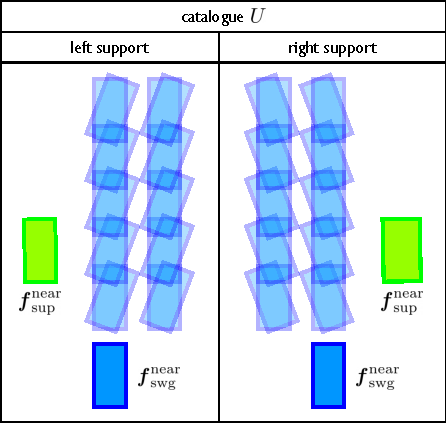
\includegraphics[width=0.65\textwidth]{figures/Primitives.pdf}
    \caption{An example catalogue $U$ of primitives, containing a finite set of
    landings for the swing foot with respect to the left or right support foot.}
    \label{fig:WoS:Primitives}
\end{figure}

Each branch joining the root of the tree to a generic vertex $v$ represents a
footstep plan $\cal P$. The sequences ${\cal S}_f$ and ${\cal S}_\varphi$ for
this plan are respectively obtained by taking along the branch the support foot
poses of all vertexes and the steps corresponding to all edges.

\medskip

\subsubsection{Footstep feasibility}
Footstep $\bff^j=(x_f^j,y_f^j,z_f^j,\theta_f^j) \in {\cal S}_f$ is
\textit{feasible} if it satisfies the following requirements:   

\begin{itemize}

\smallskip
\item[R1] $\bff^j$ is fully in contact within a single horizontal patch.

\smallskip
To guarantee this, each cell of ${\cal M}_{z}$ belonging to, or overlapping
with, the footprint at $\bff^j$ must have the same height $z_{f}^j$.
In practice, one typically uses an enlarged footprint to ensure that this
requirement will still be satisfied in the presence of small positioning errors.

\smallskip
% this is actually stance feasibility 
\item[R2] $\bff^j$ is kinematically admissible from the previous footstep
$\bff^{j-1}$ (this is actually {\em stance feasibility}).

\smallskip
%The admissible region (a submanifold of $\RealSet^3 \times SO(2)$) for placing $\bff^{j}$ next to $\bff^{j-1}$ is denoted by ${\cal A}(\bff^{j-1})$ and is defined by the following constraints:
The admissible region (a submanifold of $\RealSet^3 \times SO(2)$) for placing
$\bff^{j}$ next to $\bff^{j-1}$ is defined by the following constraints:
\begin{gather} 
-\begin{pmatrix}
\Delta_x^- \\[5pt] \Delta_y^-
\end{pmatrix}
\le
R_{j-1}^T \begin{pmatrix}
x_f^j - x_f^{j-1} \\[5pt] y_f^j - y_f^{j-1}
\end{pmatrix}
\pm \begin{pmatrix}
0 \\ \ell
\end{pmatrix}
\le
\begin{pmatrix}
\Delta_x^+ \\[5pt] \Delta_y^+
\end{pmatrix} \label{eq:WoS:XYAdmissible}\\[5pt]
-\Delta_z^- \le z_f^j - z_f^{j-1} \le \Delta_z^+
\label{eq:WoS:ZAdmissible}\\[5pt]
-\Delta_\theta^- \le \theta_f^j - \theta_f^{j-1} \le \Delta_\theta^+. \label{eq:WoS:ThetaAdmissible}
\end{gather}
Here, $R_{j-1}$ is the planar rotation matrix associated with $\theta_f^{j-1}$
and the $\Delta$ symbols are lower and upper maximum increments, see
Fig.~\ref{fig:WoS:KinCon}.

\begin{figure}
\centering
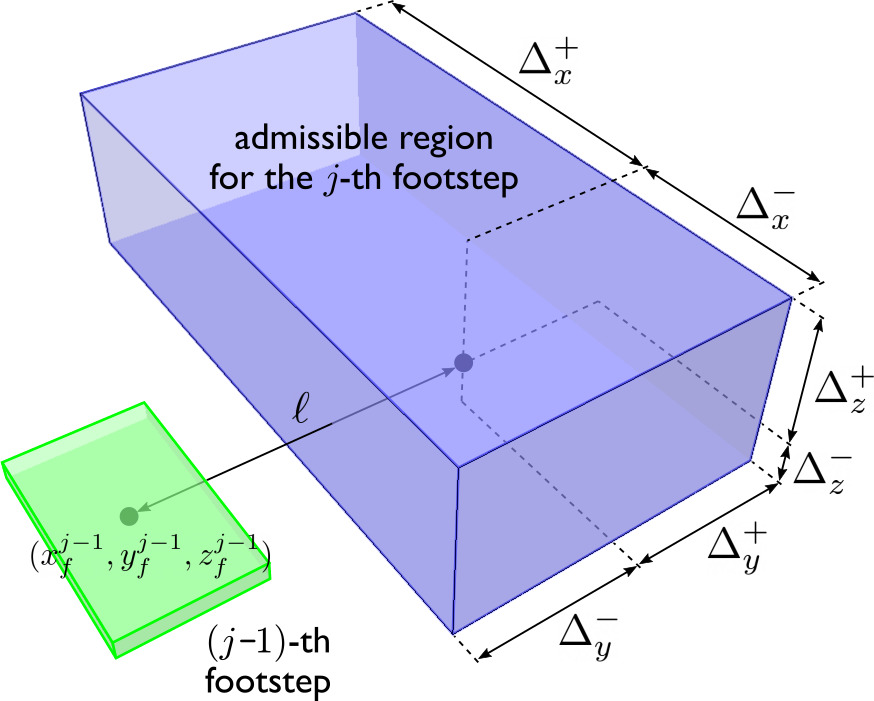
\includegraphics[width=0.6\textwidth]{figures/kinematic_limits.jpeg}
\caption{The 3D admissible region identified by the first two kinematic
constraints of requirement R2, i.e.,
eqs. (\ref{eq:WoS:XYAdmissible}-- \ref{eq:WoS:ZAdmissible}).
Footstep orientation is not represented.}
\label{fig:WoS:KinCon}
\end{figure}

% this is actually step feasibility, i.e., compatibility between successive stances
\smallskip
\item[R3] $\bff^j$ is reachable from $\bff^{j-2}$ through a collision-free
motion (this is actually {\em step feasibility}).

\smallskip
Since information about the whole-body motion of the robot is not yet available
during footstep planning (it will only be defined in the subsequent gait
generation phase), this requirement can only be tested conservatively.
In particular, we say that R3 is satisfied if ({\em i}) there exist a
collision-free swing foot trajectory $\bfvarphi^{j-2}$ from $\bff^{j-2}$ to
$\bff^{j}$ generated by the engine of
Sect.~\ref{sec:WoS:offlineCase:FP:PlannerOverview}, and ({\em ii}) a suitable
volume ${\cal B}$ accounting for the maximum occupancy of the humanoid upper
body at stance $(\bff^{j-1}, \bff^{j})$ is collision-free. More precisely,
${\cal B}$ is a vertical cylinder whose base has radius $r_b$ and center at
$(x_m, y_m, z_m + z_b)$, where $x_m$, $y_m$, $z_m$ are the coordinates of the
midpoint $\bfm$ between the footsteps and $z_b$ is a vertical offset
representing the average distance between the ground and the hip
(Fig. \ref{fig:WoS:ReqCollisionCheck}). 
Note that any nonzero height can be used for the cylinder in view of the world
of stairs assumption, which implies that ${\cal B}$ is collision-free
\footnote{Even though the volume for checking the upper body collision is chosen
conservatively, this does not guarantee obstacle avoidance because the lower
body is not considered. However, whole-body collision avoidance can be obtained
by including appropriate constraints in the kinematic controller
\cite{Escande2014IJRR}.} if each cell of ${\cal M}_z$ belonging to, or
overlapping with, its ground projection has height smaller than $z_m + z_b$.

\end{itemize}

\medskip

\subsubsection{Vertex identity, neighbors and cost}
\label{sec:WoS:offlineCase:FP:CostFunctions}
The {\em identity} of a vertex $v=(\bff_{\rm swg}, \bff_{\rm sup})$ indicates
whether  $\bff_{\rm swg}$ refers to the left ($L$) or the right ($R$) foot:
\[
{\rm id}(v)=
\begin{cases}
L\quad \mbox{if} \quad{\rm id}(v^{\rm parent}) = R \\
R\quad \mbox{if} \quad{\rm id}(v^{\rm parent}) = L,
\end{cases}
\]
where $v^{\rm parent}$ is the parent vertex of $v$.
This definition determines the identity of each vertex, once the identity of
the root is assigned.

We also define the set of {\em neighbors} of $v=(\bff_{\rm swg}, \bff_{\rm sup})$
\[
{\cal N}(v) = \{ v'=(\bff'_{\rm swg}, \bff'_{\rm sup}) \in {\cal T} : 
 \gamma(\bff_{\rm sup}, \bff'_{\rm sup}) \le r_{\rm neigh}\}
\]
where $r_{\rm neigh}$ is a threshold distance and
\begin{equation}
\gamma(\bff, \bff') = \lVert \bfp_f - \bfp_f' \rVert + k_{\gamma}|\theta_f-\theta_f'|
\label{eq:WoS:footstepToFootstepMetric}
\end{equation}
is a footstep-to-footstep metric, with $k_{\gamma}\ge 0$.

\begin{figure}
\centering
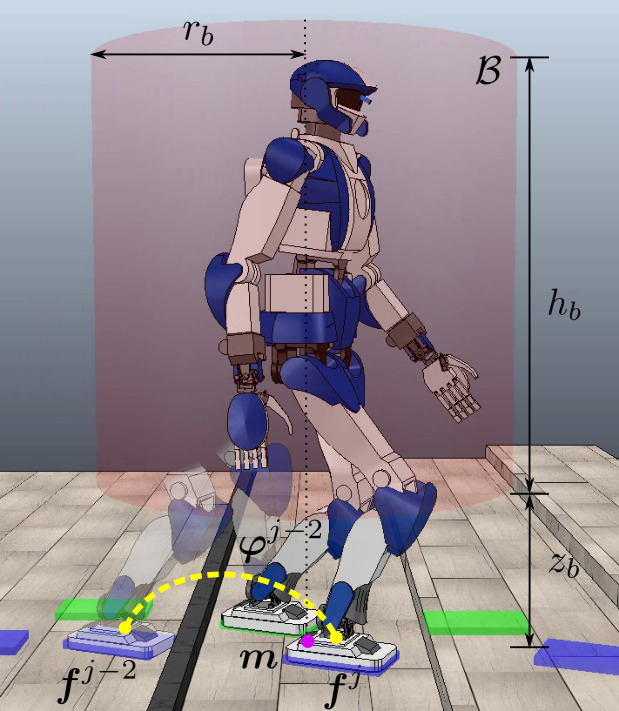
\includegraphics[width=0.55\textwidth]{figures/R3_CollisionCheck.jpeg}
\caption{Visual representation of the process for checking requirement R3.
The red cylinder accounts for the maximum occupancy of the humanoid upper body,
while the yellow line represents the swing foot trajectory.}
\label{fig:WoS:ReqCollisionCheck}
\end{figure}

Assume that the edge between two vertexes $v^a$ and $v^b$ of $\cal T$ has a
cost $l(v^a,v^b)$. 
The {\em cost} of a vertex $v$ is defined as
\[
c(v) = c(v^{\rm parent}) + l(v^{\rm parent}, v)
\]
and represents the cost of reaching $v$ from the root of $\cal T$. 
Then, the cost of a plan $\cal P$ ending at a vertex $v$ is $c({\cal P}) = c(v)$.

In particular, we will consider three possibilities for the cost of an edge.
The first is
\begin{equation}
l_1(v^a, v^b) = 1,
\label{eq:WoS:costSteps}
\end{equation}
for all edges in $\cal T$. The corresponding vertex cost will be denoted by
$c_1(v)$ and represents the length of the corresponding plan in terms of number
of edges (i.e., steps). 
    
\begin{figure}
\centering
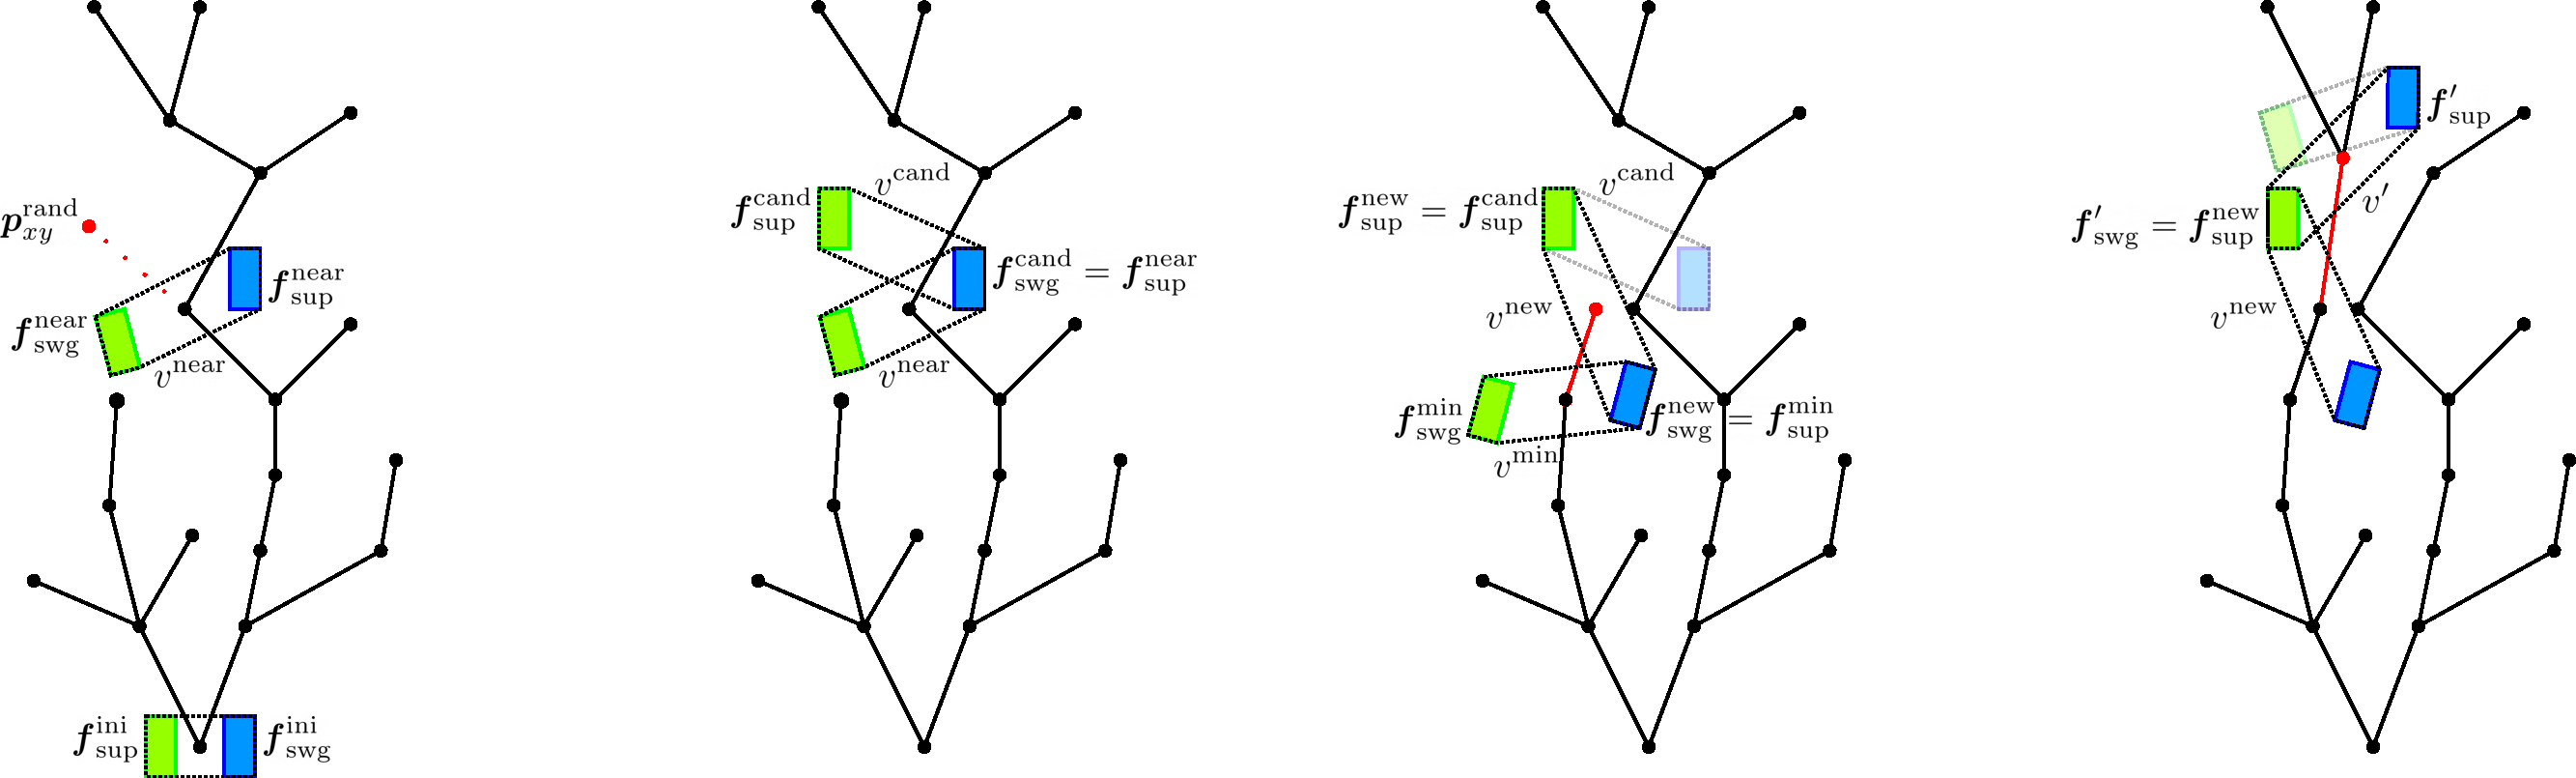
\includegraphics[width=\textwidth]{figures/FootstepPlanner.pdf}
\caption{The four steps of a generic iteration of the footstep planner.
First, a sampled point is used to select a vertex for expansion.
Then, the selected vertex is used to generate a candidate vertex to be inserted
in the tree.
In the third step, a parent for the candidate vertex is chosen.
Finally, a rewiring procedure is called to update the tree, guaranteeing that
the cost of the nodes is optimal.}
\label{fig:WoS:FootstepPlanner}
\end{figure}   
    
The second edge cost represents the net height variation of the swing foot
during a step:
\begin{equation}
l_2(v^a, v^b) = |z^b_{f, {\rm sup}} - z^a_{f, {\rm swg}}|,
\label{eq:WoS:costHeight}
\end{equation}
where $z^a_{f, {\rm swg}}$ and $z^b_{f, {\rm sup}}$ are the $z$-component of,
respectively, the swing foot at $v^a$ and the support foot at $v^b$.
The corresponding vertex cost will be denoted by $c_2(v)$ and represents the
cumulative height variation along the corresponding plan. 
    
Finally, we  also consider as edge cost
\begin{equation}
l_3(v^a, v^b) = \frac{1}{\sigma (\bff^b_{\rm sup})},
\label{eq:WoS:costClearance}
\end{equation}
where $\sigma (\bff^b_{\rm sup})$ is the {\em clearance} of the support foot
$\bff^b_{\rm sup}$ at $v^b$, defined as the distance between the representative
point of $\bff^b_{\rm sup}$ and the closest point in $\mathcal{M}_z$
w.r.t. which the absolute height variation is larger than
$\max\{\Delta_z^-, \Delta_z^+\}$\footnote{This information may be precomputed
from the elevation map ${\cal M}_z$ and stored in a clearance map.}.
This cost penalizes steps that bring the swing foot too close to a drop or to
a vertical surface leading to a contiguous higher patch,
while still allowing to approach accessible patches such as staircases.
The corresponding vertex cost, denoted by $c_3(v)$, represents the cumulative
inverse clearance along the corresponding plan.

Other kinds of cost functions can be considered. For example, one could penalize
unnecessary rotations of the next footstep with respect to the support footstep
in order to obtain smoother plans.  
In general, it may be advisable to use a weighted combination of several
optimality criteria for better practical performance. 

\medskip

\subsubsection{Algorithm}
\label{sec:WoS:offlineCase:FP:PlannerOverview}

We now describe the footstep planning algorithm for the off-line case
(Algorithm \ref{alg:FootstepPlanner}).

At the beginning, $\cal T$ is rooted at
$(\bff_{\rm swg}^{\rm ini}, \bff_{\rm sup}^{\rm ini})$, the initial stance of
the humanoid.
Then, $\cal T$ is expanded using an RRT*-like strategy. The generic iteration
consists of: selecting a vertex for expansion, generating a candidate vertex,
choosing a parent for the new vertex and rewiring the tree. These individual
steps are described in the following, see also Fig.~\ref{fig:WoS:FootstepPlanner}.

\begin{algorithm}%[!t]
	\small
	\removelatexerror
    %\caption{FootstepPlanner$(({\bff}_{\rm swg}^{\rm ini}, {\bff}_{\rm sup}^{\rm ini}), {\cal G}, {\Delta T}, {\cal M}_z)$}
	
	\caption{FootstepPlanner}
	\label{alg:FootstepPlanner}

	\KwIn{$({\bff}_{\rm swg}^{\rm ini}, {\bff}_{\rm sup}^{\rm ini}), {\cal G}, {\Delta T}, {\cal M}_z$}
	\vspace{2pt}
	\KwOut{${\cal P}^*$}
    \BlankLine
    
	$v^{\rm ini}$ $\leftarrow$ $({\bff}_{\rm swg}^{\rm ini}$, ${\bff}_{\rm sup}^{\rm ini})$\; 
	
	AddVertex$(\cal T$, $\emptyset$, $v^{\rm ini}$, $\emptyset)$\;
	
	ExpandTree$(\cal T$, ${\Delta T}$, ${\cal M}_z)$\;
	
    ${\cal P}^*$ $\leftarrow$ RetrieveBestPlan$({\cal T}, {\cal G})$\;	
    \Return{${\cal P}^*$}\;
\end{algorithm}

\begin{procedure}%[!t]
	\small
	\removelatexerror
	%\caption{ExpandTree(${\cal T}$, ${\Delta T}$, ${\cal M}_z$)}
	
	\caption{ExpandTree()}
	\label{proc:ExpandTree}

	\KwIn{${\cal T}, {\Delta T}, {\cal M}_z$}
	\vspace{2pt}
	\KwOut{none}
    \BlankLine
    
	\While{\rm \textbf{not} TimeExpired$({\Delta T})$}{
	 	$\bfp_{xy}^{\rm rand}$ $\leftarrow$ SamplePoint$()$\;
	 	$v^{\rm near}$ $\leftarrow$ NearestVertex$(\mathcal{T}, \bfp_{xy}^{\rm rand})$\;
	 	$\bff^{\rm cand}_{\rm sup}$ $\leftarrow$ GenerateCandidateFootstep$(\bff_{\rm sup}^{\rm near}, U, \mathcal{M}_z)$\;
	 	
	 	\If{\rm R1$(\bff^{\rm cand}_{\rm sup})$ \rm \textbf{and} \rm R2$(\bff^{\rm cand}_{\rm sup}, \bff^{\rm near}_{\rm sup})$}{
	 	 	$\bfvarphi^{\rm near}$ $\leftarrow$ SwingTrajectoryEngine$(\bff_{\rm swg}^{\rm near}, \bff_{\rm sup}^{\rm cand})$\;
		 	
		 	\If{\rm R3$(\bfvarphi^{\rm near}, (\bff^{\rm near}_{\rm sup}, \bff^{\rm cand}_{\rm sup}))$}{
		 	    $v^{\rm cand}$ $\leftarrow (\bff^{\rm near}_{\rm sup}, \bff^{\rm cand}_{\rm sup})$\;
		 		
		 		$\mathcal{N} \leftarrow$ Neighbors$(\mathcal{T}, v^{\rm cand})$\;
		 		
		 		$(v^{\rm min}, \bfvarphi^{\rm min}) \leftarrow$ ChooseParent$(\mathcal{T}, \mathcal{N}, v^{\rm near}, v^{\rm cand}, \bfvarphi^{\rm near})$\;
		 		
                $v^{\rm new} \leftarrow (\bff^{\rm min}_{\rm sup}, \bff^{\rm cand}_{\rm sup})$\;
		 		
		 		AddVertex$(\mathcal{T}, v^{\rm min}, v^{\rm new}, \bfvarphi^{\rm min})$\;	
		 		
		 		ReWire$(\mathcal{T}, \mathcal{N}, v^{\rm new})$\;	
		 	}   			
	 	}    
	 }
	 \Return{}\;
\end{procedure}

{\bf Selecting a vertex for expansion}: A point $\bfp_{xy}^{\rm rand}$ is
randomly selected on the $xy$-plane, and
the vertex $v^{\rm near}$ that is closest to $\bfp_{xy}^{\rm rand}$ is
identified. To this end, we define a vertex-to-point metric as
\begin{equation*}
\mu(v, \bfp_{xy}) = \lVert \bfm_{xy}(v) - \bfp_{xy} \rVert + k_{\mu} |\psi(v,\bfp_{xy})|,
\end{equation*}
where $\bfm_{xy}(v)$ represents the planar position of the midpoint between the
feet at stance $v$, $k_{\mu}$ is a positive scalar, and $\psi(v,\bfp_{xy})$ is
the angle between the robot sagittal axis (whose orientation is the average of
the orientations of the two footsteps) and the line joining $\bfm_{xy}$ to
$\bfp_{xy}$. This step corresponds to the functions SamplePoint and
NearestVertex in Procedure \ref{proc:ExpandTree}.
\hfill $\blacktriangleleft$

\begin{sloppypar}
{\bf Generating a candidate vertex}:  
After identifying the vertex
${v^{\rm near}=(\bff_{\rm swg}^{\rm near},\bff_{\rm sup}^{\rm near})}$,
a candidate footstep is first generated using the catalogue $U$
(see Fig.~\ref{fig:WoS:Primitives}). In particular, we set the support foot to
$\bff_{\rm sup}^{\rm near}$ and randomly select one element from the subset of
$U$ associated to the identity of $v^{\rm near}$, which may be $L$ (left) or
$R$ (right). Note that all elements of $U$ are chosen so as to automatically
satisfy conditions~(\ref{eq:WoS:XYAdmissible}--\ref{eq:WoS:ThetaAdmissible})
of requirement R2. Call $\bff_{\rm sup}^{\rm cand}$ the chosen candidate
footstep. The $z$ coordinate to be associated to the footstep
$\bff_{\rm sup}^{\rm cand}$ is then retrieved from ${\cal M}_{z}$, and both
the requirement R1 and the last condition~(\ref{eq:WoS:ZAdmissible}) of R2 can
now be checked.
\end{sloppypar}

To test the last requirement R3, we invoke an engine
(Procedure \ref{proc:genswgtraj}) that generates a swing foot trajectory
$\bfvarphi^{\rm near}$ from $\bff_{\rm swg}^{\rm near}$ to
$\bff_{\rm sup}^{\rm cand}$. Such engine uses a parameterized trajectory which,
given the endpoints, can be deformed\footnote{As a deformable trajectory we
used a polynomial, but other choices (e.g., B-splines and Bezier curves) are
possible.} by varying the maximum height $h$ along the motion. 
Using the elevation map and increments of $\Delta h$, the engine tries growing
values of $h$ in a certain range $[h^{\rm min}, h^{\rm max}]$ looking for a
collision-free trajectory.

If all requirements have been satisfied, a candidate vertex is generated as
$v^{\rm cand} = (\bff_{\rm swg}^{\rm cand}, \bff_{\rm sup}^{\rm cand})$, with
$\bff_{\rm swg}^{\rm cand} = \bff_{\rm sup}^{\rm near}$; however, $v^{\rm cand}$
is not added to $\cal T$ because the planner first needs to identify the best
parent for it. If any requirement among R1--R3 is violated, the current
expansion attempt is aborted and a new iteration is started.
This step corresponds to lines 4-8 in Procedure \ref{proc:ExpandTree}.
\hfill $\blacktriangleleft$

\begin{procedure}%[!t]
	\small
	\removelatexerror
	
	%\caption{SwingTrajectoryEngine($\bff^a$, $\bff^b$)}
	\caption{SwingTrajectoryEngine()}
	\label{proc:genswgtraj}

	\KwIn{$\bff^a$, $\bff^b$}
	\KwOut{$\bfvarphi^a$}
    \BlankLine

	$h$ $\leftarrow$ $h^{\rm min}$\;
	
	\While{$h \leq h^{\rm max}$}{
		$\bfvarphi^a \leftarrow$ DeformTrajectory$(\bff^a, \bff^b, h)$\;		 	
	
	   	\If{\rm CollisionFree$(\bfvarphi^a)$}{
            \Return{$\bfvarphi^a$}\;	   	
	   	}
		
	    $h \leftarrow h + \Delta h$\;
	}
			
	\Return{$\emptyset$}\;	
\end{procedure}

{\bf Choosing a parent}: Although $v^{\rm cand}$ was generated from
$v^{\rm near}$, there might be a different vertex in the tree that leads to
the same vertex with a lower cost. To find it, the planner checks for each
vertex $v' = (\bff'_{\rm swg}, \bff'_{\rm sup})\in {\cal N} (v^{\rm cand})$
whether setting $v'$ as parent of $v^{\rm cand}$ satisfies requirements R2-R3,
and whether this connection reduces the cost of $v^{\rm cand}$, that is 
\[
c(v') + l(v', v^{\rm cand}) < c(v^{\rm near}) + l(v^{\rm near}, v^{\rm cand}).
\]
The vertex $v^{\rm min} = (\bff_{\rm swg}^{\rm min}, \bff_{\rm sup}^{\rm min})$
that allows to reach $v^{\rm cand}$ with minimum cost is chosen as its parent.
If $v^{\rm min} = v^{\rm near}$, then $v^{\rm cand}$ can be added to the tree
together with the edge joining it to $v^{\rm near}$. However, if a different
parent $v^{\rm min} \neq v^{\rm near}$ is chosen, the candidate vertex
$v^{\rm cand}$ must be modified by relocating its swing footstep to the support
footstep of $v^{\rm min}$. To this end, a new vertex
$v^{\rm new} = (\bff_{\rm swg}^{\rm new}, \bff_{\rm sup}^{\rm new})$ with
$\bff_{\rm swg}^{\rm new} = \bff_{\rm sup}^{\rm min}$ and
$\bff_{\rm sup}^{\rm new} = \bff_{\rm sup}^{\rm cand}$ is generated and added
to ${\cal T}$ as child of $v^{\rm min}$. The edge between $v^{\rm min}$ and
$v^{\rm new}$ corresponds to the swing foot trajectory $\bfvarphi^{\rm min}$. 
This step corresponds to the function ChooseParent in Procedure
\ref{proc:chooseparent}.
\hfill $\blacktriangleleft$

\begin{procedure}%[!t]
	\small
	\removelatexerror
	%\caption{ChooseParent($\cal T$, $\cal N$, $v^{\rm near}$, $v^{\rm cand}$, $\bfvarphi^{\rm cand}$)}
	
	\caption{ChooseParent()}
	\label{proc:chooseparent}

	\KwIn{${\cal T}, {\cal N}, v^{\rm near}, v^{\rm cand}, \bfvarphi^{\rm cand}$}
	\vspace{2pt}
	\KwOut{$v^{\rm min}, \bfvarphi^{\rm min}$}
    \BlankLine
	
	$v^{\rm min}$ $\leftarrow$ $v^{\rm near}$\;
	$\bfvarphi^{\rm min}$ $\leftarrow$ $\bfvarphi^{\rm cand}$\;
	$c^{\rm min}$ $\leftarrow$ $c(v^{\rm near}) + l(v^{\rm near}, v^{\rm cand})$\;
	
	\ForEach{$v'$ $\in$ $\cal N$}{
    	\If{\rm R2$(\bff_{\rm sup}^{\rm cand}, \bff'_{\rm sup})$}{
    		$\bfvarphi' \leftarrow$ SwingTrajectoryEngine$(\bff'_{\rm swg}, \bff_{\rm sup}^{\rm cand})$\;
    		
    		\If{\rm R3$(\bfvarphi', (\bff'_{\rm sup}, \bff_{\rm sup}^{\rm cand}))$ \rm \textbf{and} $c(v') +l(v', v^{\rm cand}) < c^{\rm min}$}{
				$v^{\rm min}$ $\leftarrow$ $v'$\;
				$\bfvarphi^{\rm min}$ $\leftarrow$ $\bfvarphi'$\;
				$c^{\rm min}$ $\leftarrow$ $c(v') +l(v', v^{\rm cand})$\;
    		}
    	}
	}
	\Return{$(v^{\rm min}$, $\bfvarphi^{\rm min})$}\;	
\end{procedure}

{\bf Rewiring}: This final step checks whether $v^{\rm new}$ allows to reach
with a lower cost some vertex already in $\cal T$, and updates the tree
accordingly. In particular, for each
$v' = (\bff'_{\rm swg}, \bff'_{\rm sup}) \in {\cal N} (v^{\rm new})$,
the procedure checks whether setting $v'$ as a child of $v^{\rm new}$ satisfies
requirements R2-R3, and whether this connection reduces the cost of $v'$,
that is 
\[
c(v^{\rm new}) + l(v^{\rm new}, v') < c(v').
\]
If this is the case, $v'$ is modified (similarly to what was done when choosing
a parent) by relocating its swing footstep to $\bff_{\rm sup}^{\rm new}$, and
then  reconnected to $\cal T$ as a child of $v_{\rm new}$. The edge between
$v^{\rm new}$ and $v'$ corresponds to the swing foot trajectory
$\bfvarphi^{\rm new}$. Finally, for each child
$v'' = (\bff''_{\rm swg}, \bff''_{\rm sup})$ of $v'$, the swing foot trajectory
$\bfvarphi'$ from the relocated $\bff'_{\rm swg}$ to $\bff''_{\rm sup}$ is
generated and the edge between $v'$ and $v''$ is accordingly
updated\footnote{In case the engine fails to find such trajectory, the subtree
rooted at vertex $v''$ (including $v''$ itself) is simply removed from $\cal T$.}.
This step corresponds to the function ReWire in Procedure \ref{proc:rewire}.

Note that, although ${\cal N} (v^{\rm new})$ can contain ancestors of
$v^{\rm new}$, no cycle will be generated by rewiring.
In fact, it can be easily shown that any ancestor of $v^{\rm new}$ will have a
cost lower or equal than $c(v^{\rm new})$, so that it will never be set as
its child.
\hfill $\blacktriangleleft$

\begin{procedure}%[!t]
	\small
	\removelatexerror
	%\caption{ReWire($\cal T$, $\cal N$, $v^{\rm new}$)}
    \caption{ReWire()}
	\label{proc:rewire}

	\KwIn{${\cal T}, {\cal N}, v^{\rm new}$}
	\vspace{2pt}
	\KwOut{none}
    \BlankLine
			
	\ForEach{$v'$ $\in$ $\cal N$}{
        \If{\rm R2$(\bff'_{\rm sup}, \bff^{\rm new}_{\rm sup})$}{
 	 	
 	 	    $\bfvarphi^{\rm new} \leftarrow$ SwingTrajectoryEngine$(\bff_{\rm swg}^{\rm new}, \bff'_{\rm sup})$\;
	 	
    	 	\If{\rm $R3(\bfvarphi^{\rm new}, (\bff'_{\rm swg}, \bff'_{\rm sup}))$ \textbf{and} $c(v^{\rm new}) + l(v^{\rm new}, v') < c(v')$}{
                
                UpdateVertex$({\cal T}, v', (\bff_{\rm sup}^{\rm new}, \bff'_{\rm sup}))$\;
                
                UpdateEdge$({\cal T}, v^{\rm new}, v', \bfvarphi^{\rm new})$\;
                
                ${\cal V}_{\rm child} \leftarrow$ ChildVertexes$({\cal T}, v')$\;
                
                \ForEach{$v''$ $\in$ ${\cal V}_{\rm child}$}{
                    $\bfvarphi'$ $\leftarrow$ SwingTrajectoryEngine$(\bff'_{\rm swg}, \bff''_{\rm sup})$\;
                    
                    \eIf{$\bfvarphi' \neq \emptyset$}{
                        UpdateEdge$({\cal T}, v', v'', \bfvarphi')$\;
                    }
                    {
                        RemoveSubtree$({\cal T}, v'')$\; 	
                    }
    	 	    }
                 	   
    	 	}
 	    }
	}
		
	\Return\;	

\end{procedure}

\smallskip
%%%% UP TO HERE 

When the assigned time budget ${\Delta T}$ runs out, tree expansion is stopped.
The set ${\cal V}_{\rm goal}$ of vertexes $v$ such that
$\bfp_{f,{\rm sup}} \in {\cal G}$ is retrieved.
The vertex $v^*$ with minimum cost is selected as
\begin{equation}
    \label{eq:WoS:BestVertex}
    v^* = \underset{v \in {\cal V}_{\rm goal}}{\arg\!\min} \ c(v)
\end{equation}
and the corresponding footstep plan ${\cal P}^*$ is retrieved from the branch
of $\cal T$ joining the root to $v^*$.

Clearly, the larger the time budget, the better the quality of the obtained
footstep plan. %(i.e., the planner asymptotically converges to the optimal solution as the number of iterations increases).
We conjecture that our planner inherits the asymptotic optimality property of
the general RRT* algorithm \cite{Karaman2011IJRR}, although we do not have a
formal proof yet.

\subsubsection{Planning results}
\label{sec:WoS:offlineCase:FP:PlanningResults}

To assess the performance of the proposed footstep planner, we performed a
campaign of planning experiments through our C++ implementation on an Intel
Core i7-8700K CPU running at 3.7~GHz.
The tree constructed by the planner is stored in a k-d tree structure
\cite{Yershova2007ImprovingMotionPlanning}, which allows to efficiently perform
search and insertion operations.
The used robot is HRP-4, a 1.5~m tall humanoid with 34 degrees of freedom
by Kawada Robotics.

We considered the five different scenarios (see Fig. \ref{fig:WoS:Scenarios})
of different complexity described in the following.
\begin{itemize}
    \item \textit{Rod}. A thin straight obstacle, which does not provide a large enough surface to step on, must be overcome before ascending and descending a staircase. 
    \item \textit{Ditch}. A ditch can only be entered from the left and exited from the right, because the platform in the middle of it is too low to be accessed directly.
    \item \textit{Corridor}. A corridor must be exited before ascending and descending a staircase. 
    \item \textit{Maze}. A maze must be navigated, including ascending and descending a staircase, to reach the goal region.
    \item \textit{Spacious}. The goal region can be reached either by traversing a flat ground or ascending and descending a staircase.
\end{itemize}

The height of each step is 8 cm for all scenarios except \textit{Ditch} where
the height is 10 cm. 

\begin{figure}
    \centering
    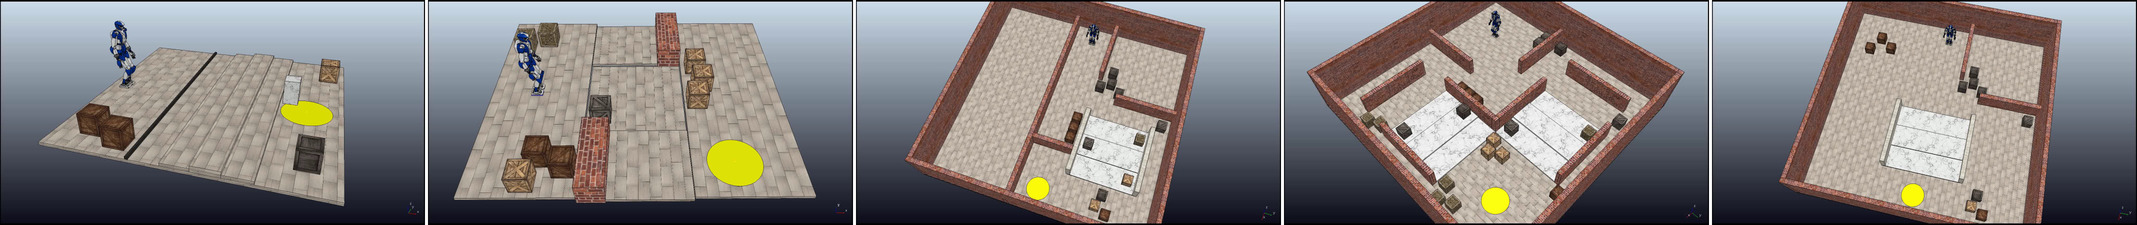
\includegraphics[width=\textwidth]{figures/PlanningScenarios.jpeg}
    \caption{The considered scenarios, from left to right: \textit{Rod}, \textit{Ditch}, \textit{Corridor}, \textit{Maze}, \textit{Spacious}.}
    \label{fig:WoS:Scenarios}
\end{figure}

\begin{figure}
    \centering
    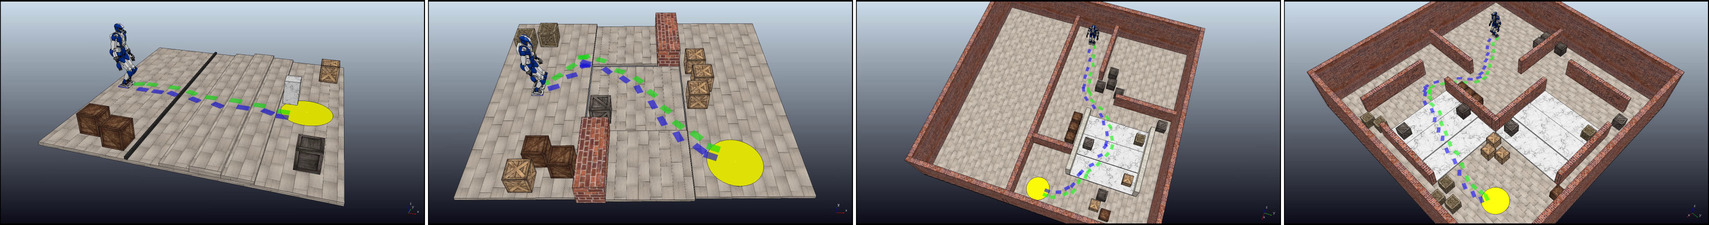
\includegraphics[width=\textwidth]{figures/ExampleResults.jpeg}
    \caption{Examples of footstep plans found in the scenarios \textit{Rod}, \textit{Ditch}, \textit{Corridor} and \textit{Maze}, respectively, when minimizing the number of steps.}
    \label{fig:WoS:ExampleResults}
\end{figure}
\begin{figure}
    \centering
    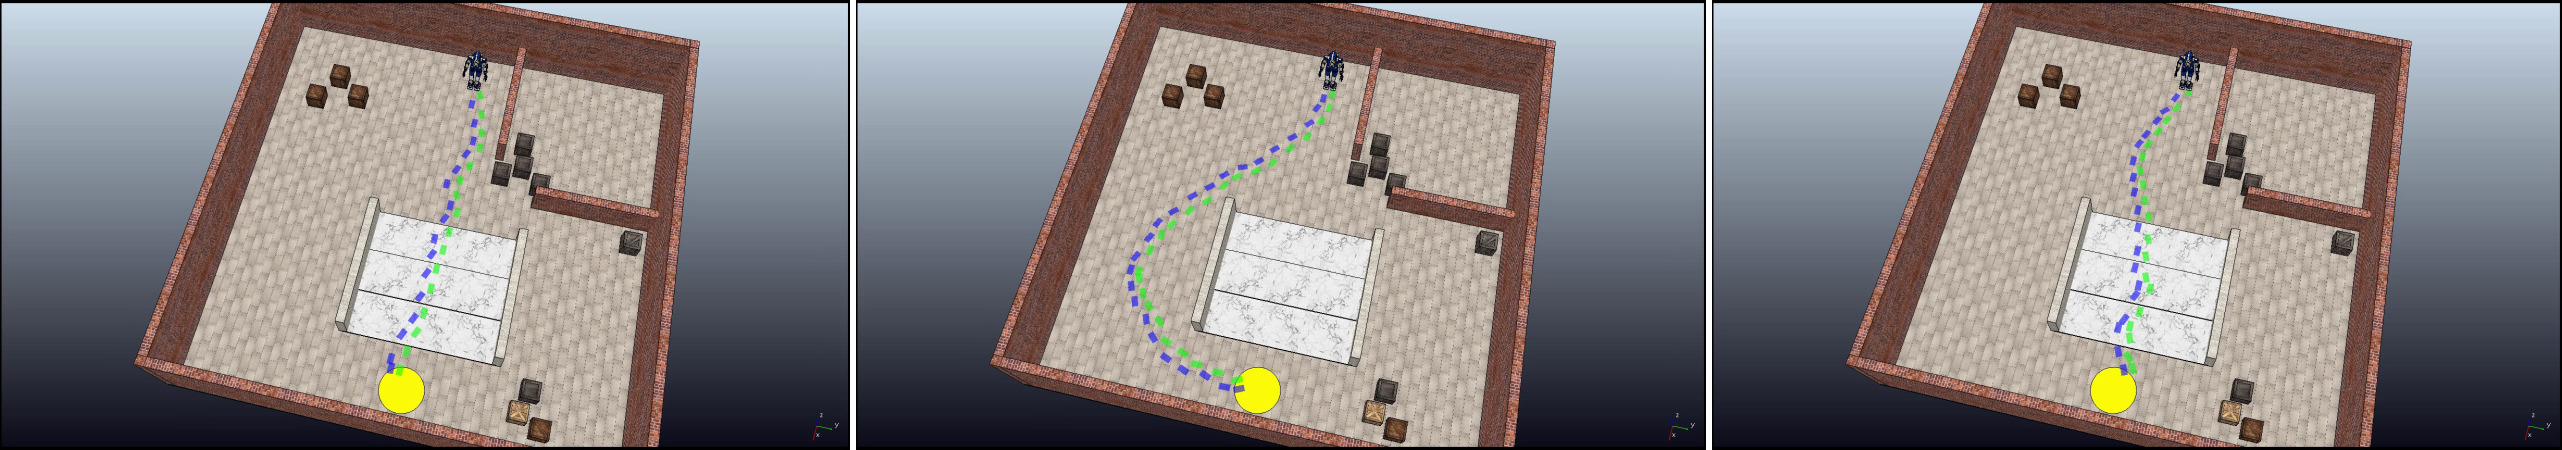
\includegraphics[width=\textwidth]{figures/ExampleResultsCompare.jpeg}
    \caption{Examples of footstep plans found in the scenario \textit{Spacious} when minimizing the number of steps, minimizing the height variation and maximizing the clearance, respectively.}
    \label{fig:WoS:ExampleResultsCompare}
\end{figure}

In all scenarios, the robot has to reach a circular goal region of radius 0.5 m.
The catalogue of primitives $U$ is generated by listing all possible
combinations of the following parameters: longitudinal displacement
$\{-0.08,0.00,0.08,0.16,0.2\}$ [m], lateral displacement $\{0.20,0.30\}$ [m]
for right support and $\{-0.20,-0.30\}$ [m] for left support, angular
displacement $\{0.00,0.40\}$ [rad] for right support and $\{0.00,-0.40\}$ [rad]
for left support (see Fig. \ref{fig:WoS:Primitives}).
In the off-line footstep planner we have set
$k_{\mu} = 1$, $k_{\gamma} = 0$, $h_{\min} = 0.02$~m, $h_{\max} = 0.24$~m,
$\Delta h = 0.02$~m, $\Delta_x^- = 0.08$~m, $\Delta_x^+ = 0.24$~m,
$\Delta_y^-=0.07$~m, $\Delta_y^+=0.07$~m, $\Delta_z^-=0.16$~m,
$\Delta_z^+=0.16$~m, $\Delta_\theta^-=-0.3$~rad, $\Delta_\theta^+=0.3$~rad,
$\ell = 0.25$~m, $z_b=0.3$~m, $h_b=1.2$~m, and $r_b=0.25$~m.
The elevation map $\mathcal{M}_z$ has a resolution of $0.02$~m.
The three quality criteria described in
Sect. \ref{sec:WoS:offlineCase:FP:CostFunctions} are considered in each scenario.

Tables \ref{tab:benchmark:off-line:steps}--\ref{tab:benchmark:off-line:clearance}
show the performance of the planner in each scenario, for different values of
the time budget, when choosing the three optimality criteria described in
Sect. \ref{sec:WoS:offlineCase:FP:CostFunctions}, respectively.
In each table, each row reports the results obtained over 100 runs on a
combination of scenario and time budget. A total of six performance indexes
are tracked and averaged over the total number of successful runs.
In particular, a run is considered unsuccessful if the planner terminates
without placing any footstep in the goal region.
Note that all unsuccessful cases are due to inappropriate time budget.
Examination of the table confirms that increasing the time budget both solves
this problem by ensuring a high success rate, and improves the quality of the
plan in terms of the average cost (Avg Cost). 
This result supports our conjecture about the asymptotic optimality of the
proposed footstep planner.

Figure \ref{fig:WoS:ExampleResults} shows the plans generated by minimizing the
number of steps in the scenarios \textit{Rod}, \textit{Ditch}, \textit{Corridor}
and \textit{Maze}.
In particular, in \textit{Rod} the plan allows to correctly pass over the thin
obstacle and walk the stairway, eventually reaching the goal region; in
\textit{Ditch} the plan reaches the left patch before traversing the low central
patches; in \textit{Corridor} the plan manages to exit the first room, reaching
the stairway and avoiding the obstacles; in \textit{Maze} the plan takes the
left path among the two available, which is the optimal one. 
Figure \ref{fig:WoS:ExampleResultsCompare} compares the plans generated in the
scenario \textit{Spacious} for each considered cost function. 
In particular, when minimizing the number of steps the plan goes straight
towards the goal region; when minimizing the height variation, the plan avoids
the stairway; when maximizing the clearance the plan first moves away from the
wall placed on the left flank of the robot at its starting configuration, and
then moves towards the goal region while keeping the other obstacles at a safe
distance.

\begin{table*}
    \centering
    \scriptsize
    \begin{tabular}{*{8}{c}}
         Scenario & Time Budget [s] & Avg Cost & Min Cost & Max Cost & Iters & Tree Size & Successes \\
        \hline
        \multirow{4}{*}{\textit{Rod}} & 1 & 22.938 & 15.000 & 35.000 & 6393.8 & 2948.7 & 96/100 \\
         & 5 & 19.810 & 15.000 & 28.000 & 21537.8 & 9863.0 & 100/100 \\
         & 10 & 18.050 & 15.000 & 25.000 & 34758.2 & 15705.5 & 100/100 \\
         & 25 & 16.600 & 15.000 & 24.000 & 62862.0 & 27944.5 & 100/100 \\
        
        \hline                                                          
        \multirow{4}{*}{\textit{Ditch}} & 1 & 40.364 & 30.000 & 51.000 & 5966.7 & 2119.5 & 33/100 \\
         & 5 & 36.450 & 27.000 & 47.000 & 18632.4 & 7100.4 & 100/100 \\
         & 10 & 33.420 & 25.000 & 42.000 & 29195.2 & 11503.3 & 100/100 \\
         & 25 & 30.940 & 25.000 & 38.000 & 52090.5 & 20755.6 & 100/100 \\  
        
        \hline                                                            
        \multirow{4}{*}{\textit{Corridor}} & 1 & 57.823 & 51.000 & 68.000 & 6131.4 & 1880.7 & 17/100 \\
         & 5 & 60.213 & 46.000 & 86.000 & 21589.9 & 5068.1 & 89/100 \\
         & 10 & 55.687 & 42.000 & 81.000 & 36426.8 & 8068.1 & 99/100 \\
         & 25 & 49.700 & 42.000 & 60.000 & 70242.7 & 14415.3 & 100/100 \\    

        \hline                                                                      
        \multirow{4}{*}{\textit{Maze}} & 1 & 74.773 & 62.000 & 89.000 & 5813.2 & 2264.9 & 22/100 \\
         & 5 & 70.949 & 54.000 & 94.000 & 21482.0 & 8695.5 & 99/100 \\
         & 10 & 65.520 & 53.000 & 80.000 & 35986.2 & 15327.2 & 100/100 \\
         & 25 & 58.240 & 50.000 & 76.000 & 67507.5 & 28891.7 & 100/100 \\ 

        \hline   
        \multirow{4}{*}{\textit{Spacious}} & 1 & 47.156 & 37.000 & 68.000 & 5749.5 & 2971.2 & 96/100 \\
         & 5 & 41.700 & 35.000 & 55.000 & 20899.7 & 10630.8 & 100/100 \\
         & 10 & 39.290 & 33.000 & 55.000 & 34665.6 & 17412.8 & 100/100 \\
         & 25 & 36.570 & 31.000 & 46.000 & 65308.0 & 31889.3 & 100/100 \\   
    
    \end{tabular}
    \caption{Performance of the off-line footstep planner when minimizing the number of steps.}
    \label{tab:benchmark:off-line:steps}
\end{table*}

\begin{table*}
    \centering
    \scriptsize
    \begin{tabular}{*{8}{c}}
         Scenario & Time Budget [s] & Avg Cost & Min Cost & Max Cost & Iters & Tree Size & Successes \\
        \hline
        \multirow{4}{*}{\textit{Rod}} & 1 & 0.450 & 0.420 & 0.480 & 6634.0 & 3186.5 & 96/100 \\
         & 5 & 0.431 & 0.420 & 0.480 & 20559.8 & 9883.2 & 100/100 \\
         & 10 & 0.425 & 0.420 & 0.480 & 31652.4 & 15140.0 & 100/100 \\
         & 25 & 0.423 & 0.420 & 0.480 & 53598.0 & 25297.7 & 100/100 \\
        
        \hline                                                          
        \multirow{4}{*}{\textit{Ditch}} & 1 & 0.640 & 0.640 & 0.640 & 6218.1 & 2294.4 & 34/100 \\
         & 5 & 0.640 & 0.640 & 0.640 & 17250.0 & 6750.3 & 100/100 \\
         & 10 & 0.640 & 0.640 & 0.640 & 25333.2 & 10171.4 & 100/100 \\
         & 25 & 0.640 & 0.640 & 0.640 & 42419.5 & 17402.7 & 100/100 \\  
        
        \hline                                                            
        \multirow{4}{*}{\textit{Corridor}} & 1 & 0.400 & 0.400 & 0.400 & 6437.1 & 2035.2 & 26/100 \\
         & 5 & 0.400 & 0.400 & 0.400 & 20834.9 & 5288.8 & 92/100 \\
         & 10 & 0.400 & 0.400 & 0.400 & 33405.4 & 8035.9 & 99/100 \\
         & 25 & 0.400 & 0.400 & 0.400 & 61279.5 & 13747.2 & 100/100 \\    

        \hline                                                                      
        \multirow{4}{*}{\textit{Maze}} & 1 & 0.480 & 0.480 & 0.480 & 6170.1 & 2455.4 & 24/100 \\
         & 5 & 0.480 & 0.480 & 0.480 & 20751.2 & 8991.1 & 99/100 \\
         & 10 & 0.480 & 0.480 & 0.480 & 33049.3 & 14808.7 & 100/100 \\
         & 25 & 0.480 & 0.480 & 0.480 & 57441.5 & 26592.6 & 100/100 \\ 
    
        \hline   
        \multirow{4}{*}{\textit{Spacious}} & 1 & 0.346 & 0.000 & 0.400 & 5961.4 & 3254.5 & 97/100 \\
         & 5 & 0.248 & 0.000 & 0.400 & 20470.8 & 11047.0 & 100/100 \\
         & 10 & 0.212 & 0.000 & 0.400 & 32485.0 & 17641.2 & 100/100 \\
         & 25 & 0.168 & 0.000 & 0.400 & 57866.5 & 30630.2 & 100/100 \\       
    
        \end{tabular}
    \caption{Performance of the off-line footstep planner when minimizing the height variation.}
    \label{tab:benchmark:off-line:height}
\end{table*}

\begin{table*}
    \centering
    \scriptsize
    \begin{tabular}{*{8}{c}}
         Scenario & Time Budget [s] & Avg Cost & Min Cost & Max Cost & Iters & Tree Size & Successes \\
        \hline
        \multirow{4}{*}{\textit{Rod}} & 1 & 30.060 & 20.556 & 58.287 & 4925.5 & 2143.6 & 92/100 \\
         & 5 & 25.480 & 18.266 & 42.102 & 16219.7 & 6785.2 & 100/100 \\
         & 10 & 23.142 & 17.586 & 36.173 & 26342.3 & 10602.8 & 100/100 \\
         & 25 & 20.331 & 17.627 & 27.902 & 48444.6 & 18275.1 & 100/100 \\
        
        \hline                                                          
        \multirow{4}{*}{\textit{Ditch}} & 1 & 78.095 & 58.308 & 98.540 & 4200.6 & 1446.2 & 10/100 \\
         & 5 & 72.377 & 54.725 & 99.004 & 13681.3 & 4456.7 & 96/100 \\
         & 10 & 64.840 & 49.282 & 83.708 & 21817.8 & 7302.6 & 100/100 \\
         & 25 & 55.466 & 44.438 & 71.903 & 39632.2 & 13139.3 & 100/100 \\  
        
        \hline                                                            
        \multirow{4}{*}{\textit{Corridor}} & 1 & 94.234 & 72.764 & 112.454 & 4538.3 & 1376.9 & 12/100 \\
         & 5 & 97.323 & 73.304 & 139.995 & 15477.9 & 3418.1 & 82/100 \\
         & 10 & 88.866 & 66.266 & 139.700 & 26354.5 & 5314.1 & 98/100 \\
         & 25 & 78.178 & 64.615 & 102.587 & 52076.3 & 9236.0 & 100/100 \\
        
        \hline                                                                      
        \multirow{4}{*}{\textit{Maze}} & 1 & 107.971 & 95.340 & 127.139 & 4374.8 & 1744.1 & 8/100 \\
         & 5 & 106.620 & 81.630 & 149.408 & 16037.0 & 5919.7 & 88/100 \\
         & 10 & 99.264 & 73.844 & 133.529 & 27154.9 & 10394.0 & 100/100 \\
         & 25 & 84.433 & 65.234 & 119.569 & 52035.2 & 19752.6 & 100/100 \\
        
        \hline   
        \multirow{4}{*}{\textit{Spacious}} & 1 & 52.476 & 32.652 & 85.874 & 4467.9 & 2286.9 & 97/100 \\
         & 5 & 47.138 & 30.160 & 70.100 & 15879.2 & 7689.2 & 100/100 \\
         & 10 & 43.535 & 28.001 & 66.777 & 26325.6 & 12425.1 & 100/100 \\
         & 25 & 38.048 & 27.357 & 57.544 & 49981.9 & 22038.9 & 100/100 \\ 
        
    \end{tabular}
    \caption{Performance of the off-line footstep planner when maximizing the minimum clearance.}
    \label{tab:benchmark:off-line:clearance}
\end{table*}

\subsection{Localization}
\label{sec:WoS:offlineCase:Localization}

The localization module is continuously fed with the RGB-D images gathered by
the head-mounted camera.
Based on such information, it is in charge of updating in real time the estimate
$\hat{\bfs}$ of the pose of the camera frame.
To this end, it uses RTAB-Map \cite{Labbe2019RTABMap}, an open source visual
SLAM library. 
In particular, the visual odometry and graph optimization tool are employed.
The first tracks the features automatically extracted from the RGB-D images,
while the second minimizes the odometry error through a graph-SLAM algorithm
and a loop closure detector.
It is worth mentioning that our architecture is independent from the specific
implementation of the localization module, hence any off-the-shelf visual SLAM
method can be employed in place of RTAB-Map (see assumption A3 in
Sect. \ref{sec:WoS:Formulation}).

Given the pose $\hat{\bfs}$ of the camera frame estimated through visual SLAM
and the measured joint positions, the direct kinematics module produces the
estimates $\hat{\bfp}_{\rm c}$ and $\hat{\bfvarphi}$ of, respectively, the
CoM position and swing foot pose. These are then provided to the gait generation
and kinematic control module to achieve closed-loop control.

\subsection{Simulations}
\label{sec:WoS:offlineCase:Simulations}
We performed simulations on the HRP-4 humanoid robot in the CoppeliaSim
environment. We tested our off-line framework in multiple environments
(Fig. \ref{fig:WoS:Scenarios}). For the gait generation module we have set
$\eta = 3.6$~s$^{-1}$, the single support duration $T_{ss}=0.6$~s, the double
support duration $T_{ds}=0.4$~s, the size of the moving box
$\tilde{d}_x^{\rm z}=\tilde{d}_y^z=d_z^z=0.05$~m, $\beta=1000$, $C=100$ and
$\delta = 0.01$~s. To solve the QP problems we used \texttt{hpipm}, which
requires less than $1$~ms to solve each QP and is thus able to run in real-time
with an ample margin.

Figure \ref{fig:WoS:offlineCase:Ditch:Snapshots} shows the robot traversing the
scenario \textit{Ditch}. The robot starts by moving to its left (first
snapshot), approaching the accessible patch (second snapshot). It then accesses
the platform in the middle correctly avoiding the obstacle (third and fourth
snapshots), eventually reaching the goal region by climbing the final two
patches (fifth and sixth snapshots).
Figure \ref{fig:WoS:offlineCase:Corridor:Snapshots} shows the robot moving
inside the scenario \textit{Corridor}. The robot first exits the room in which
it starts (first and second snapshots), approaching the stairway (third
snapshot). Then, it goes up and down the staircases avoiding the obstacles
(fourth and fifth snapshots), finally reaching the goal region (sixth snapshot).

We invite the reader to watch the video, available at
\url{https://youtu.be/BF43qUcx4gY}, which includes 
clips related to the above simulations as well as additional cases.

\begin{figure}
    \centering
    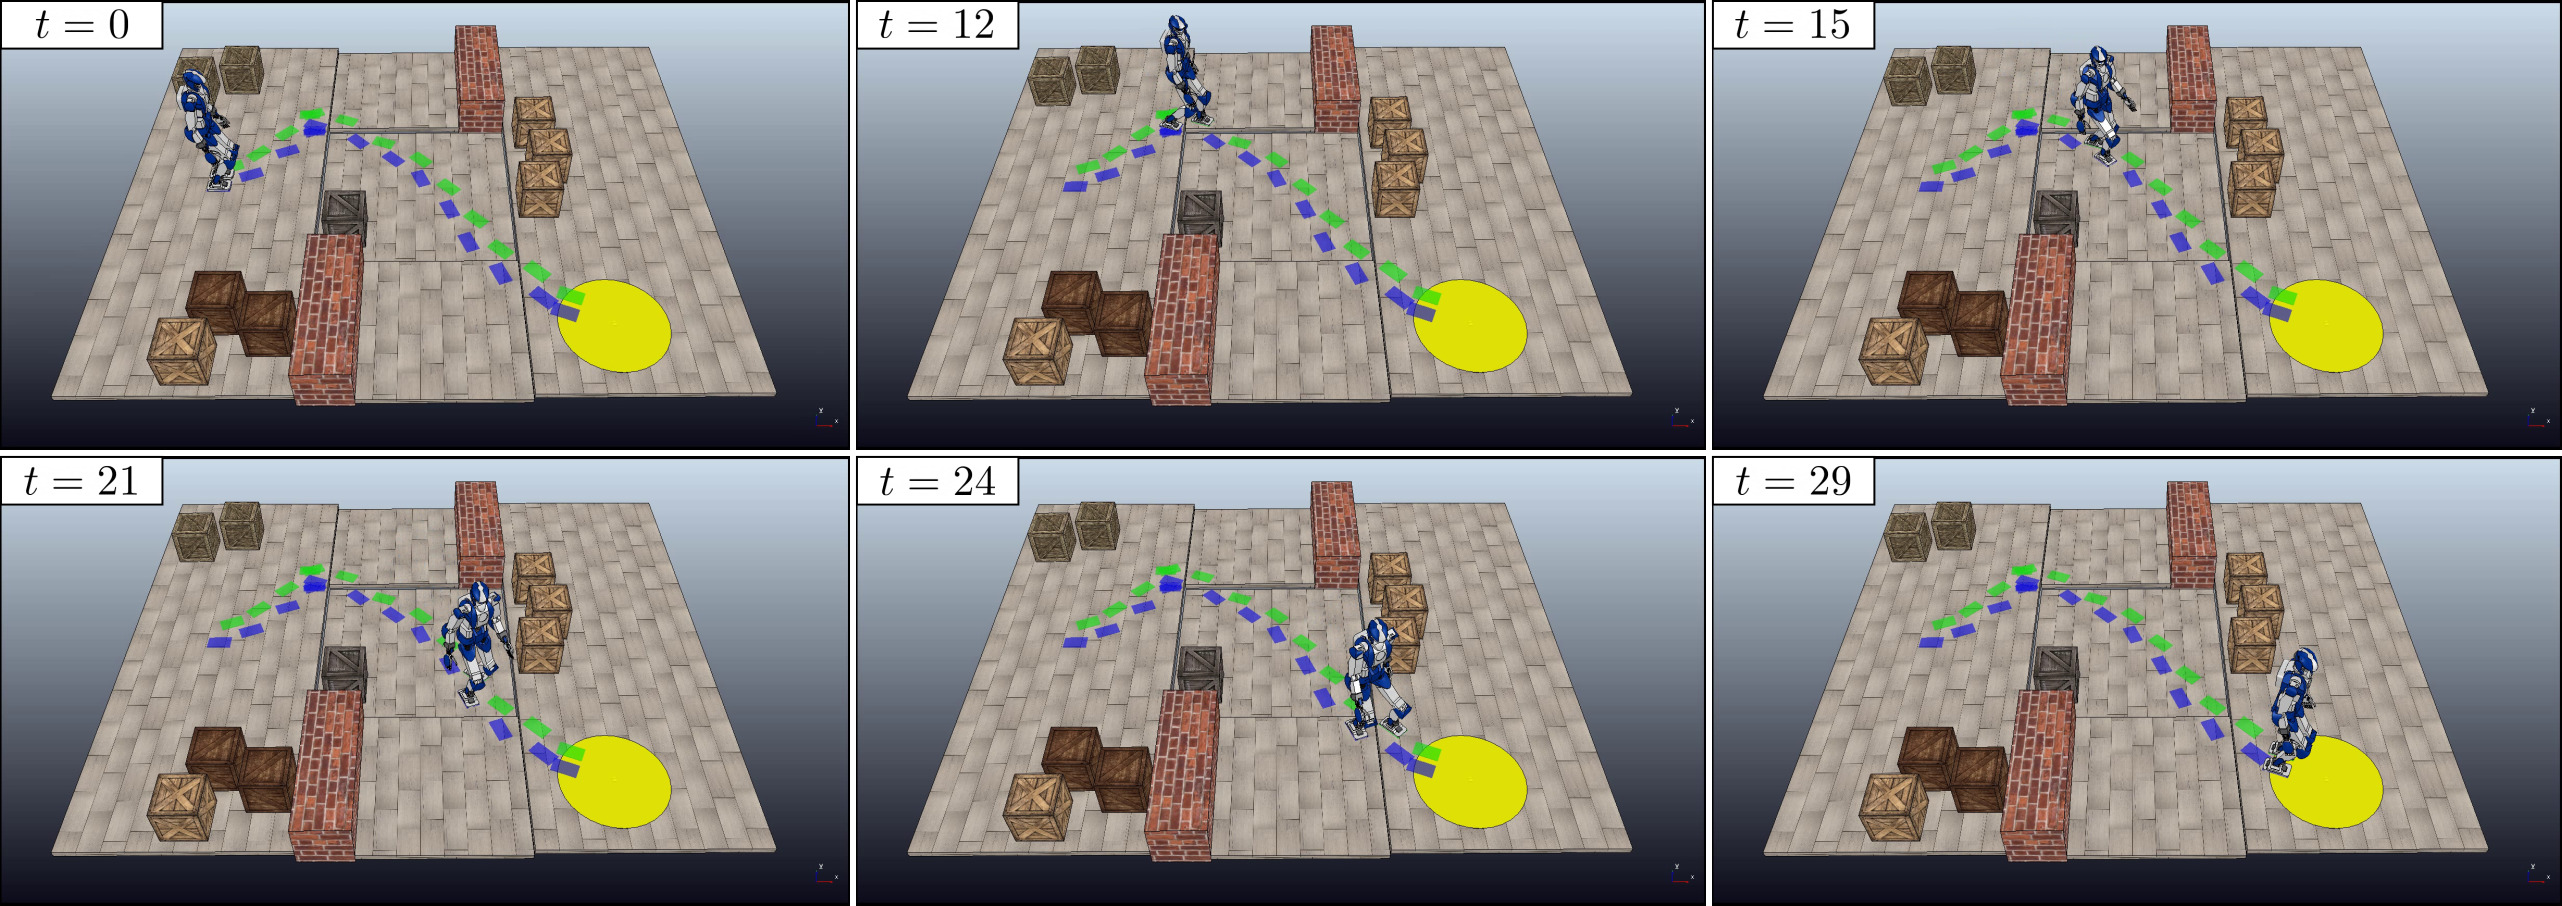
\includegraphics[width=\textwidth]{figures/OfflineDitch.jpeg}
    \caption{The robot reaches the goal going through the ditch, which can only
        be accessed from the left and exited from the right.}
    \label{fig:WoS:offlineCase:Ditch:Snapshots}
\end{figure}
\begin{figure}
    \centering
    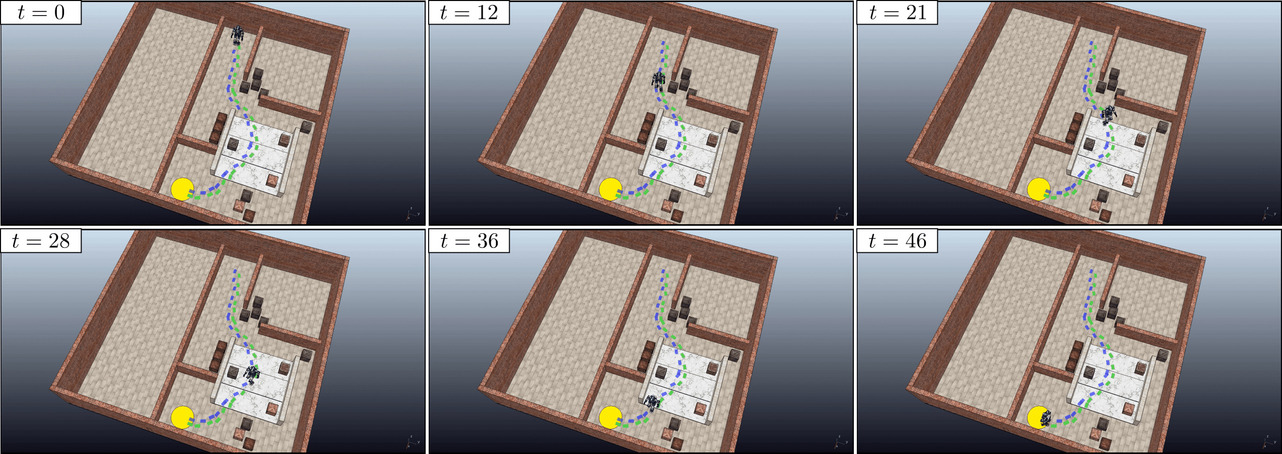
\includegraphics[width=\textwidth]{figures/OfflineCorridor.jpeg}
    \caption{The robot reaches the goal avoiding the
    corridor, climbing and descending the staircase while
    avoiding the obstacles.}
    \label{fig:WoS:offlineCase:Corridor:Snapshots}
\end{figure}


\section{The on-line case} 
\label{sec:WoS:onlineCase}

We now extend the proposed method to the on-line case.
This section starts with a description of the general architecture which,
compared to that proposed for the off-line case, includes two additional
modules, i.e., the mapping and visual task generation module, and employs a
sensor-based version of the footstep planner, which will now work on-line; all
the other modules, in particular gait generation, remain instead identical.  
Then, we describe the mentioned components and present some simulation results.

\subsection{General architecture}
\label{sec:WoS:onlineCase:GeneralArchitecture}
\begin{figure}
\centering
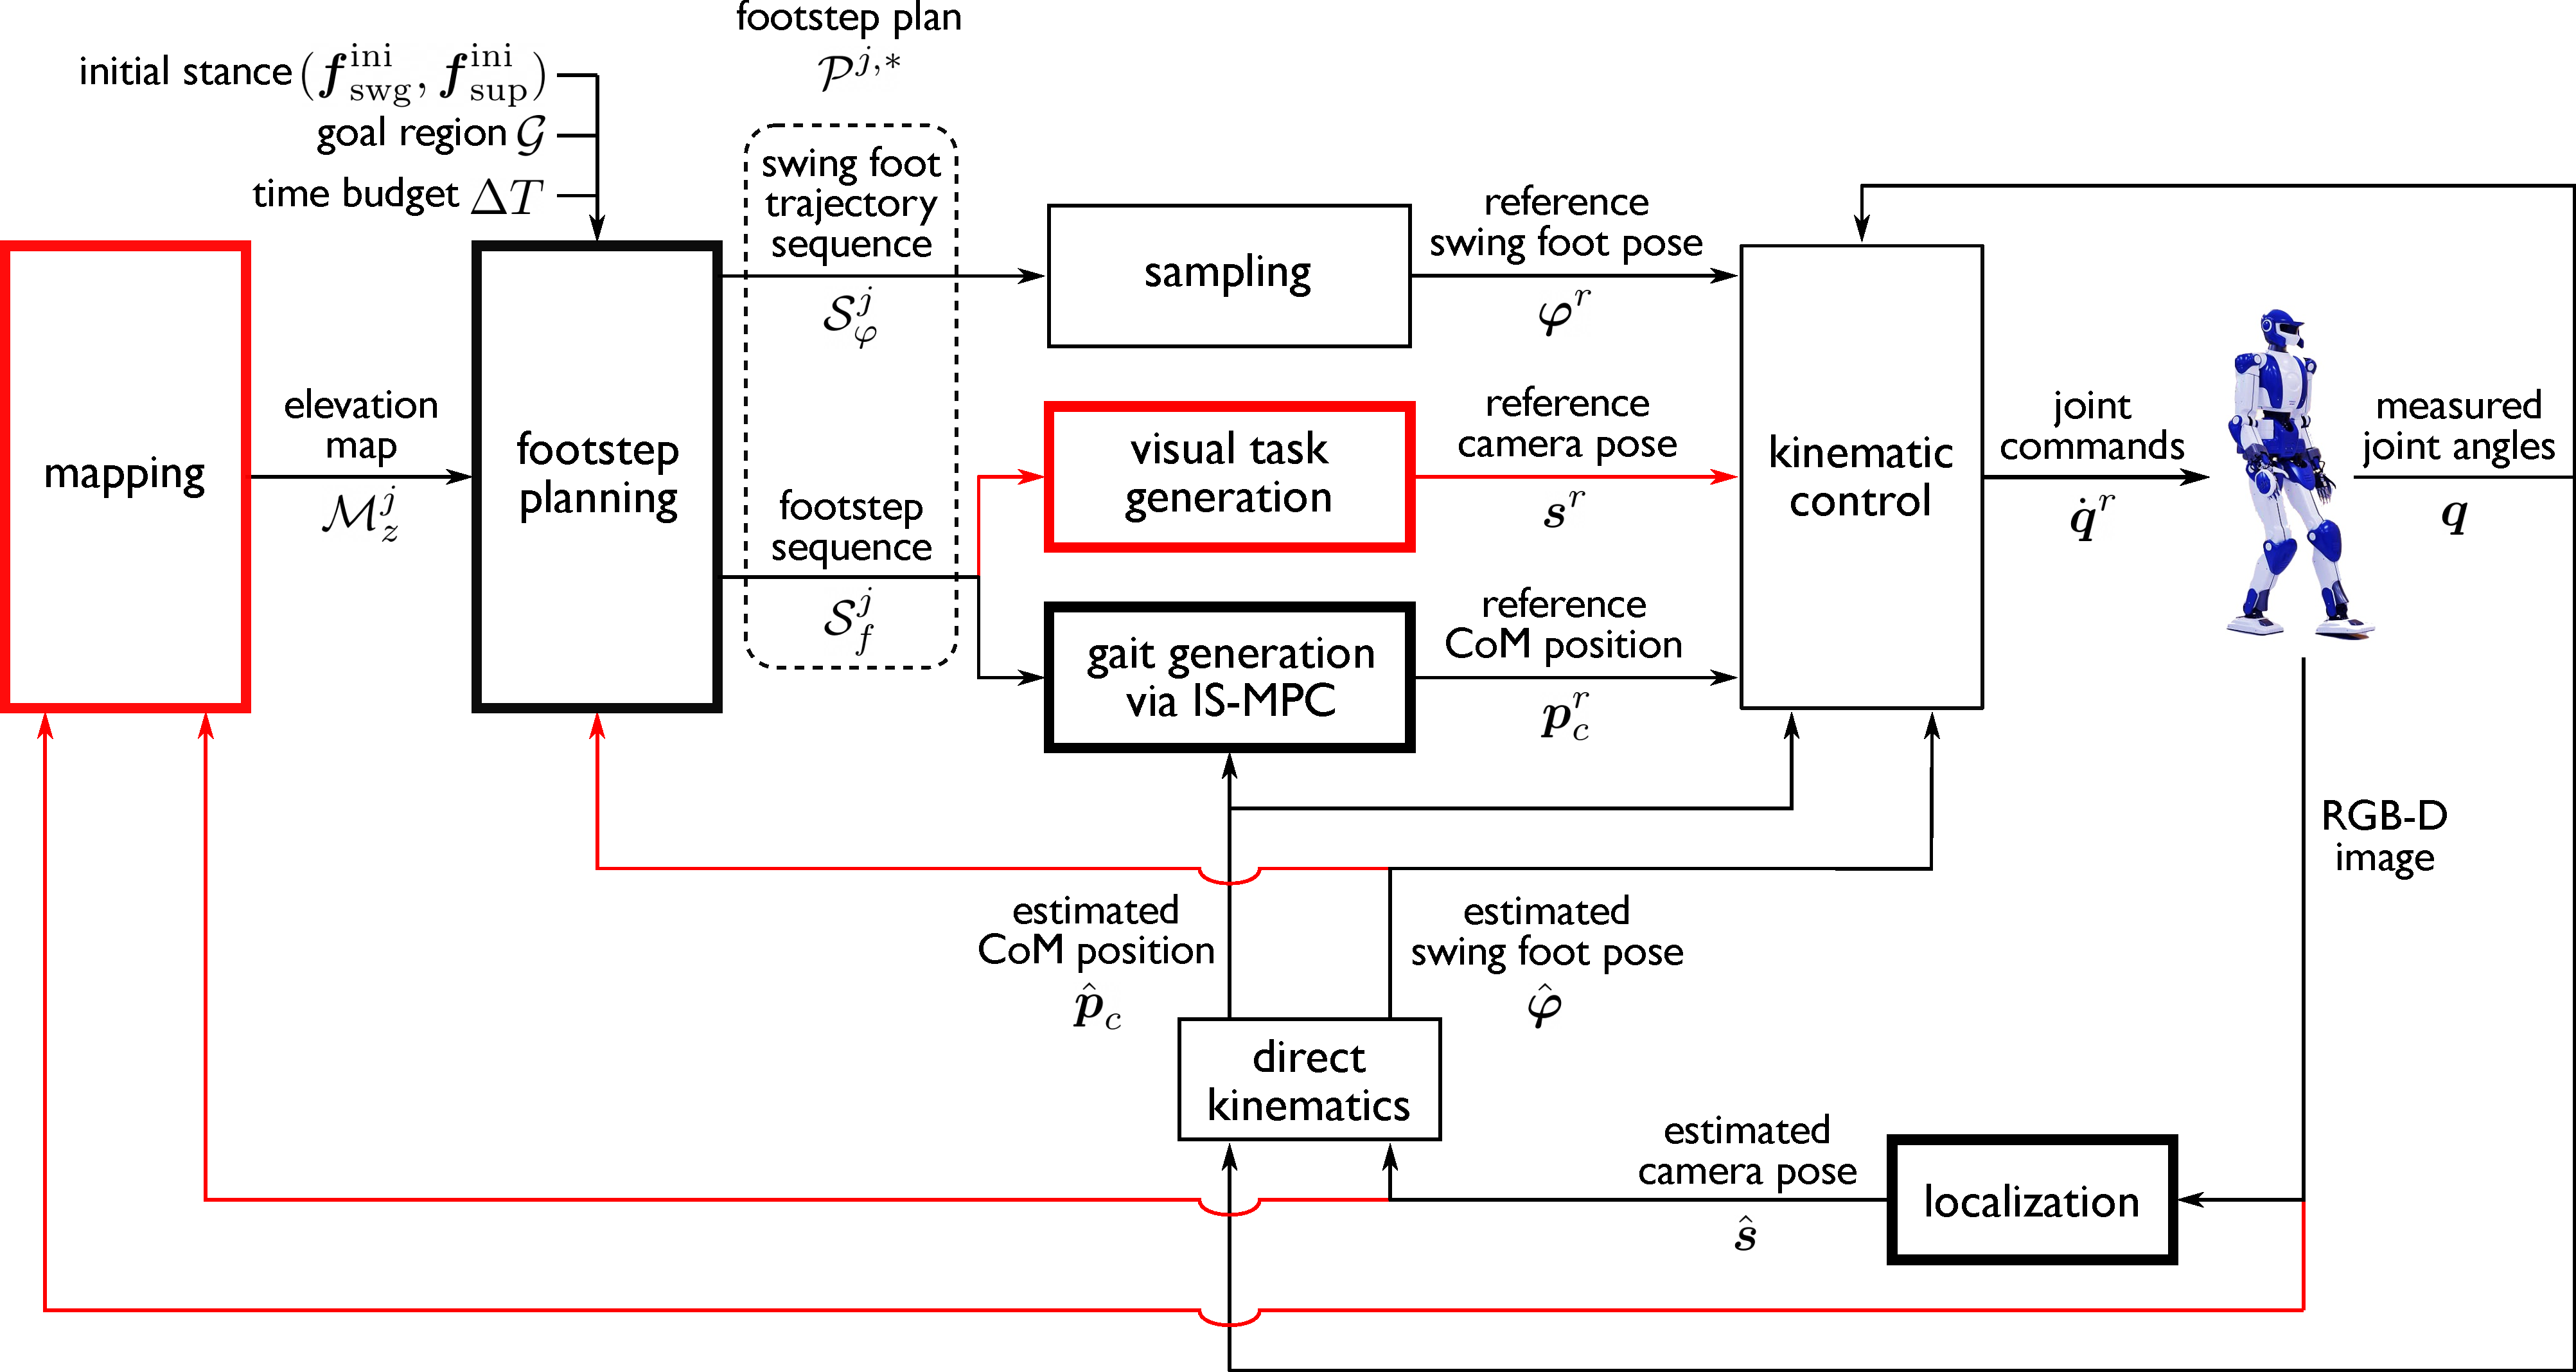
\includegraphics[width=\textwidth]{figures/BlockSchemeOnline.pdf}
\caption{Block scheme of the on-line case. The red blocks and arrows highlight
    the additional modules and signals compared to the off-line case.}
\label{fig:WoS:blockScheme2}
\end{figure}

The proposed architecture for the on-line case is given in
Fig. \ref{fig:WoS:blockScheme2}, where the additional modules and feedback
signals are shown in red.

At the beginning, the map ${\cal M}_z$ is initialized combining some limited
exogenous knowledge about the starting location of the robot and information
available by the head-mounted camera at its initial pose. Such initial map
${\cal M}_z^0$, together with the initial humanoid stance
$(\bff_{\rm swg}^{\rm ini}, \bff_{\rm sup}^{\rm ini})$, the goal region
$\cal G$ and a preassigned time budget $\Delta T$, is provided to the footstep
planner to find a first (possibly partial) footstep plan
${\cal P}^{1,*} = \{ {\cal S}_f^{1}, {\cal S}_\varphi^{1} \}$.

After this initial off-line phase, all the modules run in parallel, generating
the humanoid motions in a sensor-based, closed-loop fashion.
%
The mapping module incrementally builds the elevation map ${\cal M}_z$ using
the RGB-D images acquired by the humanoid while walking and the estimate
$\hat{\bfs}$ of the camera pose produced by the localization module.
To account for changes in ${\cal M}_z$ and take advantage of newly acquired
information, the footstep plan is on-line updated and/or extended by repeatedly
invoking the footstep planner at every step of the humanoid, with the ultimate
objective of reaching $\cal G$. 

More precisely, consider the generic timestamp $t_s^j$, i.e., the beginning of
the $j$-th step.
Let $(\hat{\bff}_{\rm swg}^{j}, \hat{\bff}_{\rm sup}^{j})$ be the current
stance, with $\hat{\bff}_{\rm swg}^{j}$ and $\hat{\bff}_{\rm sup}^{j}$ the
estimates of the swing and support foot poses at $t_s^j$, and
${\cal P}^{j,*} = \{ {\cal S}_f^{j}, {\cal S}_\varphi^{j} \}$ be the current
footstep plan -- computed during the previous ($(j-1)$-th) step -- where the
sequences of footstep placements and associated swing trajectories are defined
as
\begin{gather*}
    {\cal S}_f^j = \{\bff^{j|j}, \dots, \bff^{j+n|j}\}, \\
    {\cal S}_\varphi^j = \{\bfvarphi^{j|j}, \dots, \bfvarphi^{j+n-2|j}\}
\end{gather*}
with their generic elements $\bff^{j+i|j}$ and $\bfvarphi^{j+i|j}$ denoting,
respectively, the $(j+i)$-th footstep and trajectory produced by the $j$-th
planner invocation, $\bff^{j|j} \approx \hat{\bff}_{\rm swg}^{j}$,
$\bff^{j+1|j} \approx \hat{\bff}_{\rm sup}^{j}$ and the last footstep
$\bff^{j+n|j}$ henceforth referred to as \textit{subgoal}.
Also, let $(\bff_{\rm swg}^{j+1}, \bff_{\rm sup}^{j+1})$ be the stance that the
humanoid is supposed to achieve at $t_s^{j+1} = t_s^j + T_s^j$, with
$\bff_{\rm swg}^{j+1} = \hat{\bff}_{\rm sup}^{j}$ and
$\bff_{\rm sup}^{j+1} = \bff^{j+2|j}$, after performing the swing trajectory
$\bfvarphi^{j|j}$ having duration $T_s^j$.
%
Then, during the time interval $[t_s^j, t_s^{j+1})$, motion execution and
footstep planning take place simultaneously as follows.
\begin{itemize}
    \item At any time instant $t \in [t_s^j, t_s^{j+1})$, the current reference
        position $\bfp_{\rm c}^r$ of the CoM is produced by the gait generator,
        based on the sequence ${\cal S}_f^j$, similarly to the off-line case;
        the current reference pose $\bfvarphi^r$ of the swing foot is obtained
        by sampling the trajectory $\bfvarphi^{j|j}$; moreover, the visual task
        generator produces the reference pose $\bfs^r$ of the camera frame,
        given its current estimate $\hat{\bfs}$ and the sequence ${\cal S}_f^j$,
        that allows to direct the gaze towards the subgoal extracted from
        ${\cal S}_f^j$, and then to enlarge ${\cal M}_z$ in the area of the
        current destination. 
        References $\bfp_{\rm c}^r$, $\bfvarphi^r$, $\bfs^r$, together with
        their estimates $\hat{\bfp}_{\rm c}$, $\hat{\bfvarphi}$, $\hat{\bfs}$,
        are passed to the kinematic controller to compute the joint commands
        $\dot{\bfq}^r$ for the robot.
    \item At $t_s^j$, the footstep planner is invoked providing in input the
        stance $(\bff_{\rm swg}^{j+1}, \bff_{\rm sup}^{j+1})$, the goal region
        $\cal G$, a time budget equal to $T_s^j$, and the elevation map
        ${\cal M}_z^j$ currently available by the mapping module.
        At $t_s^{j+1}$, the planner returns a new footstep plan
        ${\cal P}^{j+1,*} = \{ {\cal S}_f^{j+1}, {\cal S}_\varphi^{j+1}\}$, where
        the sequences ${\cal S}_f^{j+1}$ and ${\cal S}_\varphi^{j+1}$ are
        defined similarly to ${\cal S}_f^{j}$ and
        ${\cal S}_\varphi^{j}$, $\bff^{j+1|j+1} = \bff_{\rm swg}^{j+1}$ and
        $\bff^{j+2|j+1} = \bff_{\rm sup}^{j+1}$. 
        The first element $\bfvarphi^{j+1|j+1}$ of ${\cal S}_\varphi^{j+1}$ will
        define the next ($(j+1)$-th) step of the humanoid. 
\end{itemize}

Note that, while the footstep planner will make use of a fixed map
$\mathcal{M}_z^j$ during the time interval $[t_s^j, t_s^{j+1})$, the map
$\mathcal{M}_z$ will continuously be updated by the mapping module during the
same time interval, which will generally provide a different map
$\mathcal{M}_z^{j+1}$ for the next invocation of the planner.

Clearly, in the on-line case, only the quality of the partial footstep plans can
be accounted for, ultimately leading to an overall plan that is globally suboptimal. 

\subsection{Mapping}
\label{sec:WoS:onlineCase:MappingModule}
At the generic time instant, the mapping module receives in input the last RGB-D
image acquired by the head-mounted camera and the current estimate $\hat{\bfs}$
of the camera pose produced by the localization module. 
It is responsible for integrating such newly acquired information into the
elevation map $\mathcal{M}_z$.

First, the depth data extracted from the RGB-D image are used to construct a
point cloud.
Then, the latter is given in input, together with the estimate $\hat{\bfs}$ and
a sensor noise model, to Elevation Mapping
\cite{Fankhauser2018ProbabilisticTerrainMapping}, an open source framework
designed for rough terrain mapping; this accordingly updates a local
(limited around the robot)
representation of the environment in the form of a 2.5D grid map (see
Assumption A1). Finally, such local map is integrated into $\mathcal{M}_z$ in
order to maintain a global representation of the explored area of the environment.

The mapping module, at the time $t_s^j$ of the generic $j$-th invocation of
the footstep planner, provides it with a copy $\mathcal{M}_z^j$ of the available
map $\mathcal{M}_z$.
Meanwhile, during the planner operation, the map $\mathcal{M}_z$ is continuously
updated through the process described above.

\subsection{Sensor-based footstep planning}
\label{sec:WoS:onlineCase:FootstepPlanner}
This module consists in a sensor-based version of the footstep planner proposed
in Sect. \ref{sec:WoS:offlineCase:FootstepPlanner} which works using the
knowledge about the environment incrementally acquired by the robot during motion. 
We now describe the footstep planning algorithm for the on-line case (Algorithm
\ref{alg:AnytimeFootstepPlanner}).

\begin{algorithm}%[!t]
	\small
	\removelatexerror
    %\caption{SensorBasedFootstepPlanner$(({\bff}_{\rm swg}^{j+1}, {\bff}_{\rm sup}^{j+1}), {\cal G}, {\Delta T}^j, {\cal M}_z^j)$}
	
	\caption{SensorBasedFootstepPlanner}
	\label{alg:AnytimeFootstepPlanner}

	\KwIn{$({\bff}_{\rm swg}^{j+1}, {\bff}_{\rm sup}^{j+1}), {\cal G}, {\Delta T}^j, {\cal M}_z^j$}
	\vspace{2pt}
	\KwOut{${\cal P}^{j+1,*}$}
    \BlankLine

    $({\cal T}^{j+1}, v^{\rm root})$ $\leftarrow$ InitializeTree$({\cal T}^j, ({\bff}_{\rm swg}^{j+1}, {\bff}_{\rm sup}^{j+1}))$\; 
	
    ${\cal V}_{\rm child}$ $\leftarrow$ ChildVertexes$({\cal T}^{j+1}, v^{\rm root})$\;
	\ForEach{$v'$ $\in$ ${\cal V}_{\rm child}$}{
        UpdateTree$({\cal T}^{j+1}, v', {\cal M}_z^j)$\;
    } 	

	ExpandTree$({\cal T}^{j+1}, {\Delta T}^j - {\Delta T}_{\rm e}, {\cal M}_z^j)$\;

	${\cal P}^{j+1,*}$ $\leftarrow$ RetrieveBestPlan$({\cal T}^{j+1}, {\cal G})$\;
    \Return{${\cal P}^{j+1,*}$}\;
\end{algorithm}

The input data for the $j$-th invocation of the footstep planner are the next
robot stance $(\bff_{\rm swg}^{j+1}, \bff_{\rm sup}^{j+1})$, the goal region
$\cal G$, the time budget ${\Delta T}^j$ and the elevation map ${\cal M}_z^j$. 
Given an optimality criterion, the footstep planner returns the best footstep
plan ${\cal P}^{j+1,*}$, found within ${\Delta T}^j$, either leading to $\cal G$
or terminating in proximity of the frontier of ${\cal M}_z^j$.
The latter case is typical whenever $\cal G$ is not included in ${\cal M}_z^j$,
e.g., due to occlusions or simply being placed far from the robot.

The planning algorithm builds a tree $\mathcal{T}^{j+1}$ reusing portions of
the tree $\mathcal{T}^{j}$ built up to the previous invocation. 
In this tree, vertexes and edges are defined as described in
Sect. \ref{sec:WoS:offlineCase:FootstepPlanner}, with the only difference that
a vertex $v = (\bff_{\rm swg}, \bff_{\rm sup})$ can contain a support footstep
$\bff_{\rm sup}$ whose $z$-coordinate is unspecified, indicating that
${\cal M}_z^j$ does not provide enough information (in a sense formally defined
in the following) about the ground under the foot at $\bff_{\rm sup}$. 
Vertexes with this characteristic represent stances located on the frontier of
${\cal M}_z^j$ and thus indicate possible direction for further exploration of
the environment. 
%
The generic invocation consists of: initializing, updating and expanding the
tree. These individual steps are described in the following.

{\bf Initializing}: The vertex $v^{\rm root} = (\bff_{\rm swg}^{\rm root}, \bff_{\rm sup}^{\rm root})$ of $\mathcal{T}^{j}$ that is closest to $(\bff_{\rm swg}^{j+1}, \bff_{\rm sup}^{j+1})$ is identified. To this end, we define a stance-to-stance metric as
\begin{equation}
    \label{eq:WoS:metricIdentifyRoot}
    \zeta(v, v') = \gamma(\bff_{\rm swg}, \bff'_{\rm swg}) + \gamma(\bff_{\rm sup}, \bff'_{\rm sup}) 
\end{equation}
where $\gamma(\cdot)$ is the footstep-to-footstep metric defined in
(\ref{eq:WoS:footstepToFootstepMetric}).
The subtree of $\mathcal{T}^{j}$ rooted at $v^{\rm root}$ is extracted
(including $v^{\rm root}$ itself) and represents the initial version of
$\mathcal{T}^{j+1}$.
To match the stance that the humanoid is supposed to reach at the end of the
simultaneously executed step, $v^{\rm root}$ is modified by relocating
$\bff_{\rm swg}^{\rm root}$ to $\bff_{\rm swg}^{j+1}$ and
$\bff_{\rm sup}^{\rm root}$ to $\bff_{\rm sup}^{j+1}$.
This step corresponds to Procedure \ref{proc:InitializeTree}.
\hfill $\blacktriangleleft$
\begin{procedure}%[!t]
	\small
	\removelatexerror
	%\caption{InitializeTree(${\cal T}^j$, ($\bff_{\rm swg}^{j+1}$, $\bff_{\rm sup}^{j+1}$))}
	\caption{InitializeTree()}
	\label{proc:InitializeTree}

	\KwIn{${\cal T}^j, (\bff_{\rm swg}^{j+1}, \bff_{\rm sup}^{j+1}))$}
	\vspace{2pt}
	\KwOut{${\cal T}^{j+1}, v^{\rm root}$}
    \BlankLine
	
	$v^{\rm root}$ $\leftarrow$ NearestVertex$({\cal T}^j, (\bff_{\rm swg}^{j+1}, \bff_{\rm sup}^{j+1}))$\;
	
	${\cal T}^{j+1}$ $\leftarrow$ ExtractSubtree$({\cal T}^j, v^{\rm root})$\;
	
	UpdateVertex$({\cal T}^{j+1}, v^{\rm root}, (\bff_{\rm swg}^{j+1}, \bff_{\rm sup}^{j+1}))$\;
	
    \Return{$({\cal T}^{j+1}, v^{\rm root})$}\;
	
\end{procedure}

{\bf Updating}: At this point, requirements R1--R3 are satisfied by
construction in $\mathcal{T}^{j+1}$ according to the previous map
$\mathcal{M}_z^{j-1}$.
Then, R1--R3 must now be checked in $\mathcal{T}^{j+1}$ using the most recent
map $\mathcal{M}_z^{j}$, consequently updating vertexes and edges in order to
satisfy them.
To this end, we perform a pre-order traversal of $\mathcal{T}^{j+1}$ as
described in the following.

When a vertex $v = (\bff_{\rm swg}, \bff_{\rm sup})$ is visited, it is
modified\footnote{This modification is not made on $v^{\rm root}$ as it
corresponds to the stance that the robot must reach at the end of the
simultaneously executed step.} by relocating its swing footstep to the support
footstep $\bff_{\rm sup}^{\rm parent}$ of its parent
$v^{\rm parent} = (\bff_{\rm swg}^{\rm parent}, \bff_{\rm sup}^{\rm parent})$,
and setting the $z$ coordinate $z_{f, \rm sup}$ of $\bff_{\rm sup}$ according
to $\mathcal{M}_z^{j}$.
In particular, consider the cells of ${\cal M}_z^j$ belonging to, or
overlapping with, the footprint at $\bff_{\rm sup}$; let $n_{\rm k}$ and
$n_{\rm u}$ be the number of these cells whose height is known and unknown,
respectively. If the rate of cells with known height is larger than a predefined
threshold $\bar{n}$, i.e.,
\begin{equation*}
    \frac{n_{\rm k}}{n_{\rm k} + n_{\rm u}} > \bar{n},    
\end{equation*}
$z_{f, \rm sup}$ is set to the average value of the $n_{\rm k}$ known heights. 
Otherwise, $z_{f, \rm sup}$ is left unspecified.

Once $v$ has been updated, requirements R1--R3 are checked similarly to what
was done in the off-line case, with the only two differences described in the
following.
\begin{itemize}
    \item If $z_{f, \rm sup}$ is unspecified, requirements R1--R3 are checked
        conjecturing that it is equal to the $z$-component $z_{f, \rm swg}$ of
        $\bff_{\rm swg}$.
    %
    \item Requirement R1 is considered satisfied if for each of the $n_{\rm k}$
        known heights, the net variation from $z_{f, \rm sup}$ does not exceed
        a predefined threshold $\bar{z}$, i.e.,
        \begin{equation*}
            |z_{\rm k} - z_{f, \rm sup}| \leq \bar{z}.
        \end{equation*}
        with $z_{\rm k}$ the generic known height among the $n_{\rm k}$ available.
\end{itemize}

If any requirement among R1--R3 is violated, vertex $v$ is removed from
$\mathcal{T}^{j+1}$, along with its descendants.
Otherwise, the edge connecting $v$ to $v^{\rm parent}$ is replaced by the
trajectory $\bfvarphi^{\rm parent}$ generated while checking R3; the set
${\cal V}_{\rm child}$ of child vertexes of $v$ is retrieved, and the procedure
is recursively invoked on them. 
To guarantee on-line performance and save time to be used for expanding
$\mathcal{T}^{j+1}$, recursion is stopped on vertexes having a maximum depth
$\bar{\kappa}$.
This step corresponds to Procedure \ref{proc:UpdateTree}.
\begin{procedure}%[!t]
	\small
	\removelatexerror
	
    %\caption{UpdateTree(${\cal T}^{j+1}$, $v$, ${\cal M}_z^j$)}
    \caption{UpdateTree()}
	\label{proc:UpdateTree}

	\KwIn{${\cal T}^{j+1}, v, {\cal M}_z^j$}
	\vspace{2pt}
	\KwOut{none}
    \BlankLine
	
	$v^{\rm parent}$ $\leftarrow$ ParentVertex$({\cal T}^{j+1}, v)$\;
    
    $z_{f, \rm sup}$ $\leftarrow$ DetermineFootstepHeight$(\bff_{\rm sup}, {\cal M}_z^j)$\;
    
    UpdateVertex$({\cal T}^{j+1}, v, (\bff_{\rm sup}^{\rm parent}, (x_{f, \rm sup}, y_{f, \rm sup}, z_{f, \rm sup})))$\;
    
    \eIf{\rm R1$(\bff_{\rm sup})$ \rm \textbf{and} \rm R2$(\bff_{\rm sup}$, $\bff^{\rm parent}_{\rm sup})$}{
 	 	$\bfvarphi^{\rm parent}$ $\leftarrow$ SwingTrajectoryEngine$(\bff_{\rm swg}^{\rm parent}, \bff_{\rm sup})$\;
	 	
	 	\eIf{\rm R3$(\bfvarphi^{\rm parent}, (\bff_{\rm swg}, \bff_{\rm sup}))$}{
            UpdateEdge$({\cal T}^{j+1}, v^{\rm parent}, v, \bfvarphi^{\rm parent})$\;
            
            \If{\rm Depth$({\cal T}^{j+1}, v))$ = $\bar\kappa$}{
                \Return\;    	
            } 	
            
            ${\cal V}_{\rm child}$ $\leftarrow$ ChildVertexes$({\cal T}^{j+1}, v)$\;
            \ForEach{$v'$ $\in$ ${\cal V}_{\rm child}$}{
                UpdateTree$({\cal T}^{j+1}, v', {\cal M}_z^j)$\;
            }
             	   
	 	} 
	 	{
	 	    RemoveSubtree$({\cal T}^{j+1}, v)$\; 	
	 	}
 	}
	{
 	    RemoveSubtree$({\cal T}^{j+1}, v)$\; 	
 	}
	 
    \Return\;   
	
\end{procedure}
\hfill $\blacktriangleleft$

{\bf Expanding}: Once $\mathcal{T}^{j+1}$ has been updated, it can be further
expanded in the map $\mathcal{M}_z^j$.
Let ${\Delta T}_{\rm e}$ be the time elapsed since the beginning of the current
invocation of the footstep planner, i.e., the time spent in initializing and
updating $\mathcal{T}^{j+1}$.
The expansion of $\mathcal{T}^{j+1}$ works iteratively as described in
Sect. \ref{sec:WoS:offlineCase:FP:PlannerOverview} using the remaining portion
of the time budget ${\Delta T}^j - {\Delta T}_{\rm e}$ and the map
$\mathcal{M}_z^j$, with the following modifications.
\begin{itemize}
    \item The choice of the $z$-coordinate for a candidate footstep
        $\bff_{\rm sup}^{\rm cand}$ and the check of requirements R1--R3 are
        done exactly as when updating a generic vertex. 
    \item A vertex whose support footstep has unspecified $z$-coordinate
        cannot be set as parent of another vertex.
        Then, such vertexes are excluded both when selecting the vertex
        $v^{\rm near}$ for an expansion attempt and when choosing a parent for
        a candidate vertex $v^{\rm cand}$. \hfill $\blacktriangleleft$
\end{itemize} 

Similarly to the off-line case, when the assigned time budget ${\Delta T}^j$
runs out, tree expansion is stopped and the set ${\cal V}_{\rm goal}$ of
vertexes $v$ such that $\bfp_{f,{\rm sup}} \in {\cal G}$ is retrieved.
%
If ${\cal V}_{\rm goal}$ is not empty, the vertex $v^*$ with minimum cost is
selected as in (\ref{eq:WoS:BestVertex}).
%
Otherwise, if ${\cal V}_{\rm goal}$ is empty, the planner retrieves the set
${\cal V}_{\rm fron}$ containing all vertexes of $\mathcal{T}^{j+1}$ having at
least one child vertex whose support footstep has unspecified $z$-coordinate.
In practice, vertexes in ${\cal V}_{\rm fron}$ contain stances located in
proximity of the frontier of the current map $\mathcal{M}_z^j$.
Then, the vertex $v^*$ is selected as
\begin{equation}
    \label{eq:WoS:BestVertexSubgoal}
    v^* = \underset{v \in {\cal V}_{\rm fron}}{\arg\!\min} \ c(v)+g(v)
\end{equation}
where $g(v)$ represents the \textit{cost-to-go} of vertex $v$, i.e., a
lower-bound on the minimum cost to reach $\mathcal{G}$ from $v$.
A possible choice for $g(v)$ when minimizing the number of steps along the
plan will be described in Sect. \ref{sec:WoS:onlineCase:Simulations}.

Finally, the footstep plan ${\cal P}^{j+1,*}$ is retrieved from the branch of
$\mathcal{T}^{j+1}$ joining the root to $v^*$. 
Clearly, if ${\cal V}_{\rm goal}$ is not empty, ${\cal P}^{j+1,*}$ will be a
complete footstep plan leading to $\mathcal{G}$; otherwise, ${\cal P}^{j+1,*}$
will be a partial footstep plan leading in the direction of an unknown area of
the environment whose exploration is considered useful -- according to the
adopted cost-to-go -- to proceed towards $\mathcal{G}$. 

\subsection{Visual task generation}
\label{sec:WoS:onlineCase:VisualTaskGeneration}
At any time instant during the execution of the generic $j$-th step, given the
current estimate $\hat{\bfs}$ of the camera pose and the subgoal $\bff^{j+n|j}$,
which is readily extracted from the current sequence $\mathcal{S}_f^j$ of
footstep placements, the visual task generator is in charge of producing a
suitable reference $\bfs^r$ of the camera pose which aims at directing the gaze
towards the current destination of the robot. 
The rationale beyond this choice is that, since the current footstep plan
terminates in an area on the frontier of the map $\mathcal{M}_z$ that is
considered promising for goal-oriented exploration of the environment, looking
in the direction of $\bff^{j+n|j}$ allows to enlarge the map in that particular
area. In principle, whenever possible, this will privilege further extension of
the footstep plan in that promising direction.

To compute $\bfs^r$, one possibility consists in adopting an image-based visual
servoing scheme \cite{Chaumette2016VisualServoing}. 
In particular, one may define a virtual feature in the image plane of the camera
at $\hat{\bfs}$ associated to the representative point $\bfp_f^{j+n|j}$ of the
subgoal footstep $\bff^{j+n|j}$.
Then, the reference pose $\bfs^r$ of the camera frame can be computed so as to
keep such feature at the center of the image plane.

The produced reference pose $\bfs^r$ is passed to the kinematic controller
which, in practice, only controls the camera yaw and pitch angles.

\subsection{Simulations}
\label{sec:WoS:onlineCase:Simulations}

\begin{figure}
    \centering
    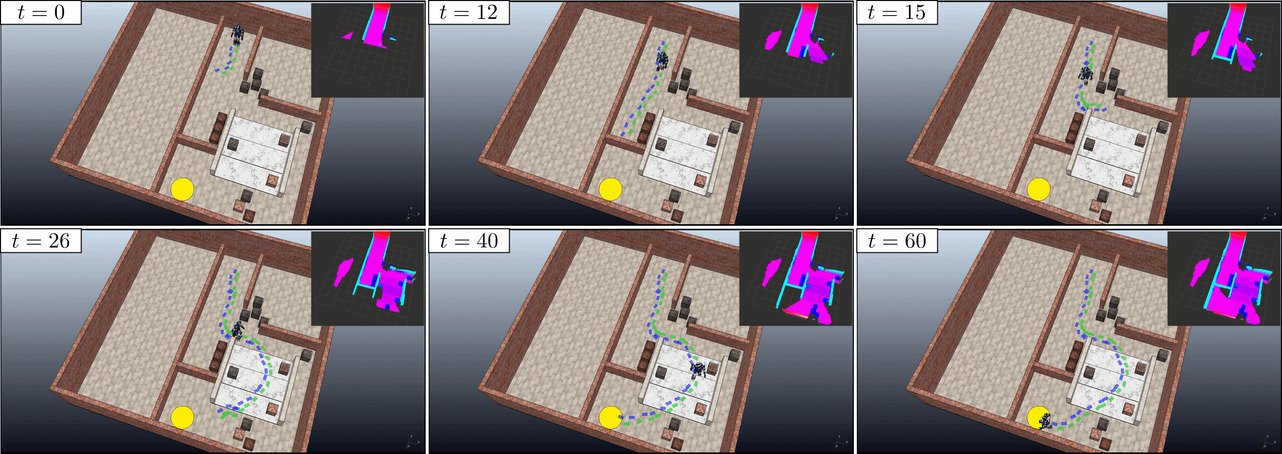
\includegraphics[width=\textwidth]{figures/OnlineCorridor.jpeg}
    \caption{The on-line footstep planner in the scenario \textit{Corridor} minimizing the number of steps. Here the planner finds a footstep sequence of 54 steps.}
    \label{fig:WoS:onlineCase:Corridor:Simulation}
\end{figure}
\begin{figure}
    \centering
    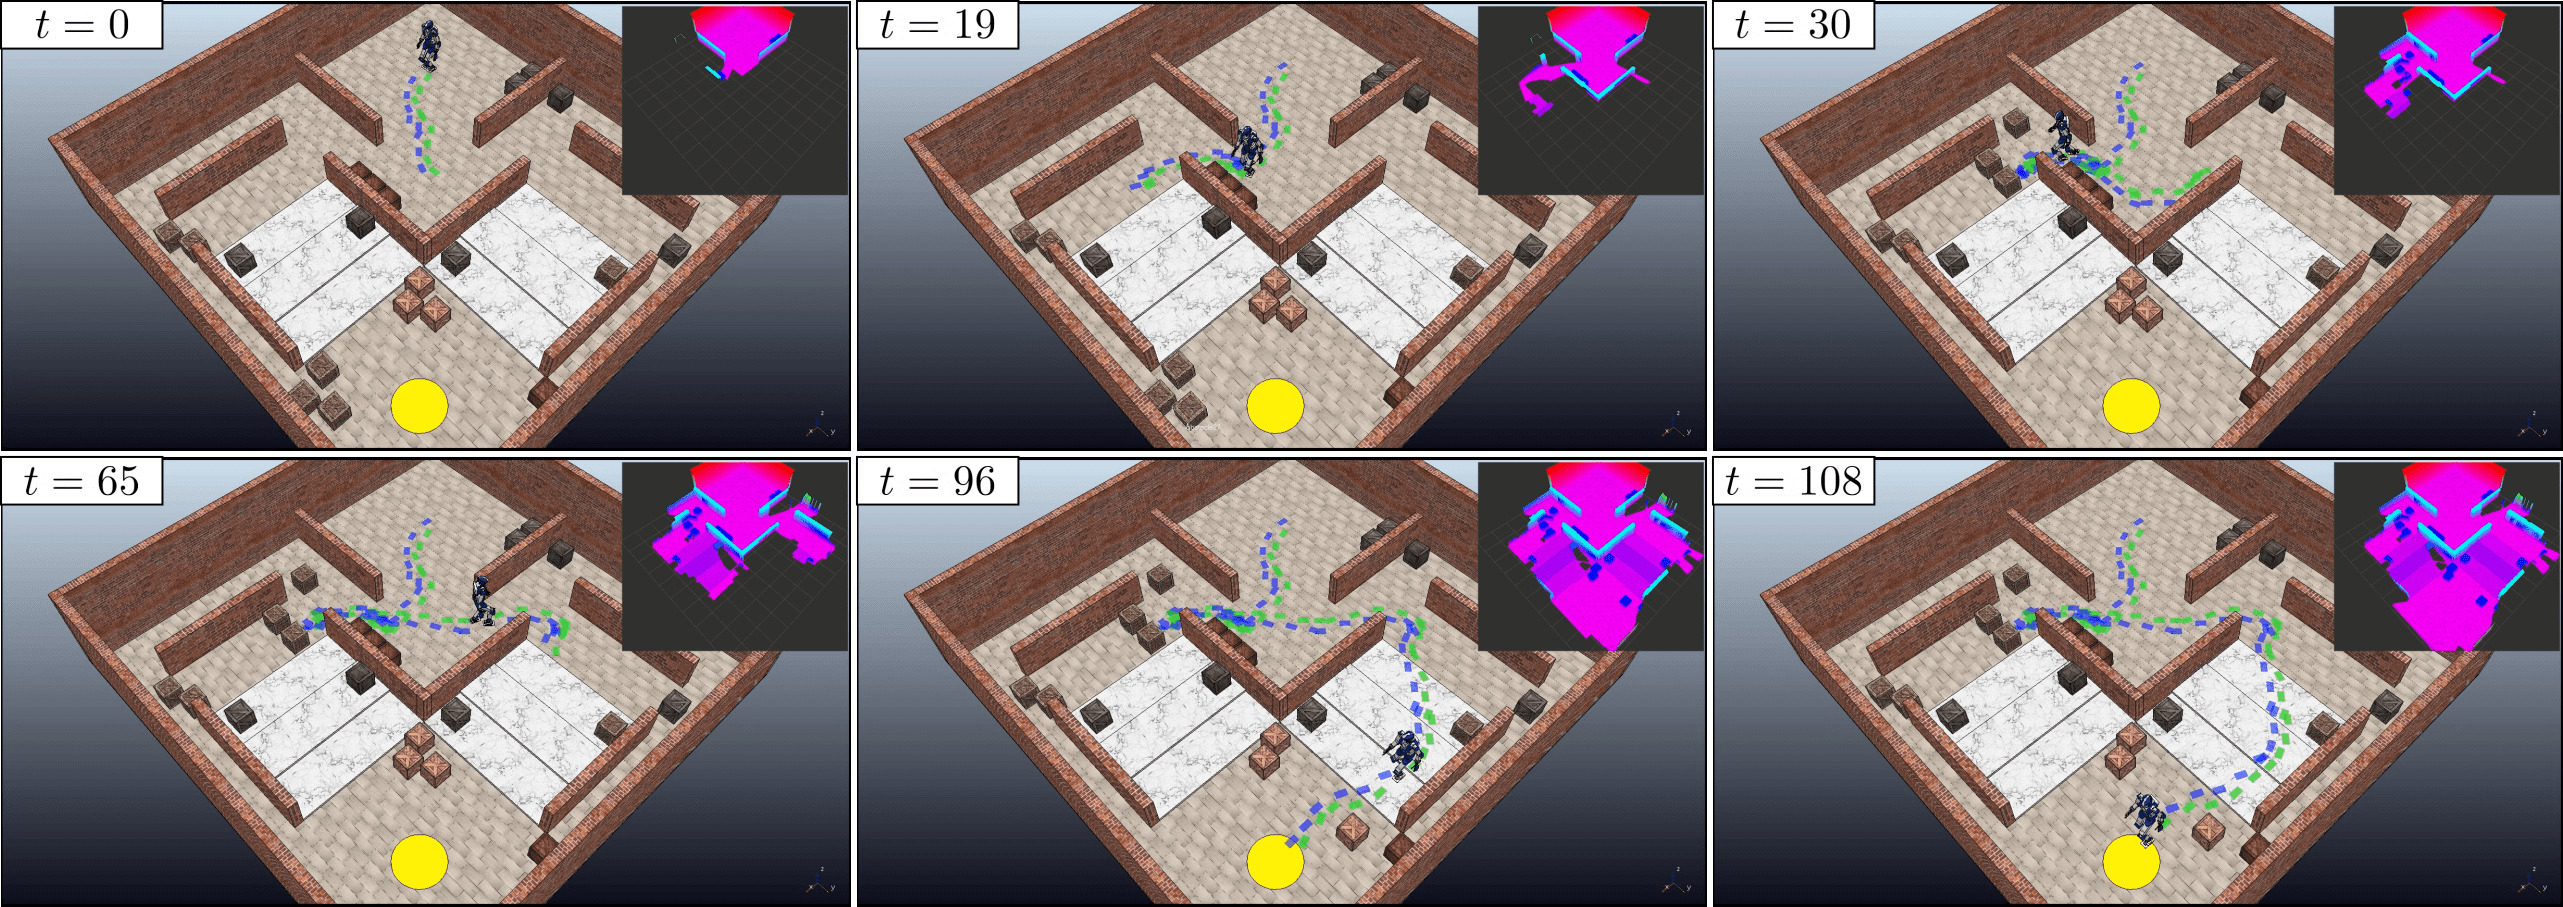
\includegraphics[width=\textwidth]{figures/OnlineMazeDynamic.jpeg}
    \caption{The on-line footstep planner in the environment \textit{Maze} minimizing the number of steps. The environment is dynamic, namely the elevation map can be changed by moving obstacles around. Here the planner finds a footstep sequence of 106 steps.}
    \label{fig:WoS:onlineCase:MazeDynamic:Simulation}
\end{figure}
\begin{figure}
    \centering
    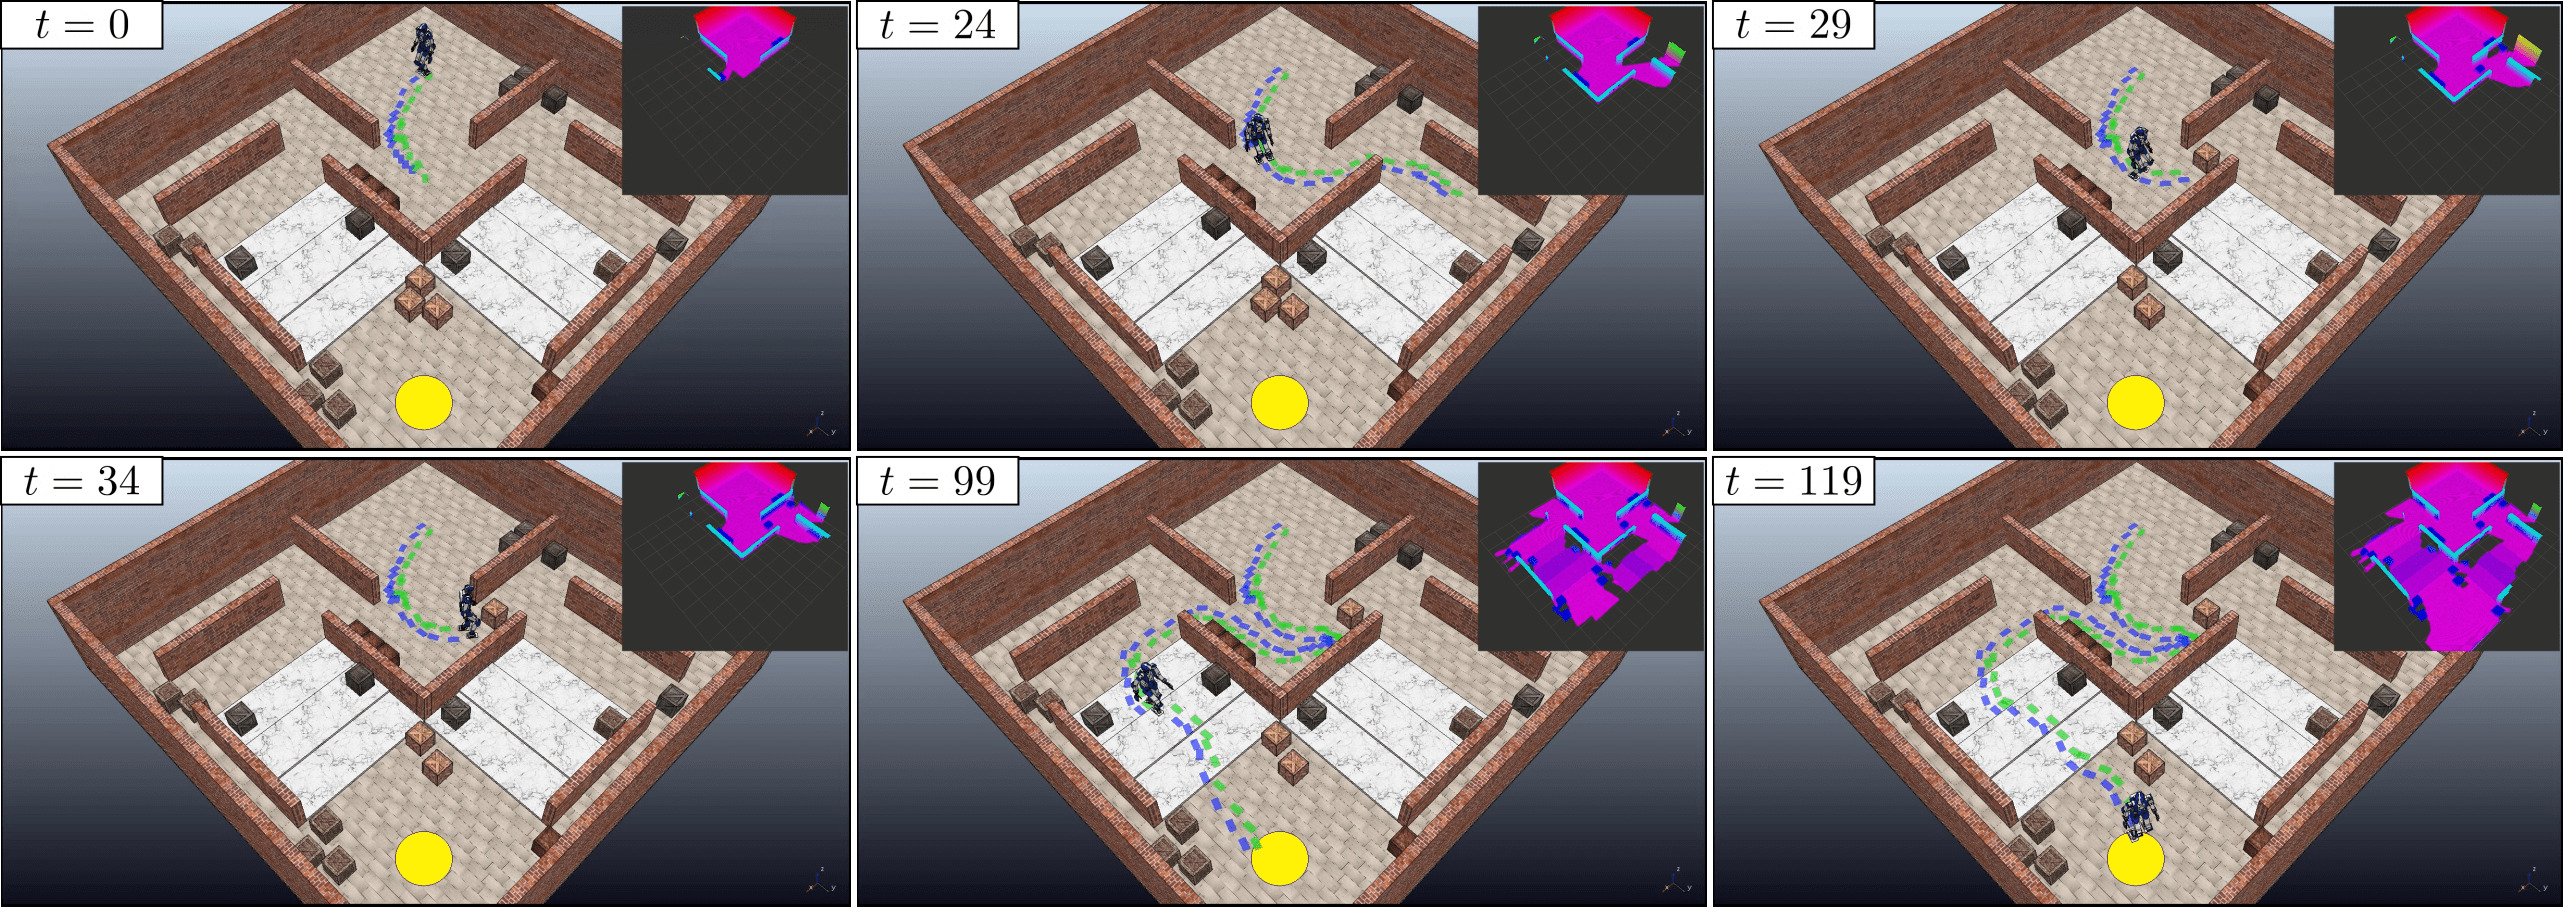
\includegraphics[width=\textwidth]{figures/OnlineMazeStopandgo.jpeg}
    \caption{The on-line footstep planner in the dynamic environment \textit{Maze} minimizing the number of steps. Here the planner finds a footstep sequence of 103 steps.}
    \label{fig:WoS:onlineCase:MazeStopAndGo:Simulation}
\end{figure}

In this section we present simulations obtained with the discussed architecture
for the on-line case. Parameters are set to the same values of
Sect. \ref{sec:WoS:offlineCase:Simulations}, with the only exception of setting
$k_\gamma = 1$ in \eqref{eq:WoS:footstepToFootstepMetric} when used in
\eqref{eq:WoS:metricIdentifyRoot}, $\bar{n}=0.9$, $\bar{z}=0.02$ and
${\bar{\kappa}}=5$. For each $j$-th invocation of the footstep planner the time
budget $\Delta T^j$ is set to $T_{ss}+T_{ds}$. In all performed simulations,
the quality criteria considered by the footstep planner is the number of steps,
while the \textit{cost-to-go} of each vertex $v$ is an underestimation of the
number of steps needed to reach the goal region $\mathcal{G}$ from the double
support configuration specified by $v$. This value is computed as the distance
between the position of the support foot specified by $v$ and $\mathcal{G}$,
divided by the longest step among the catalogue of primitives $U$. 

Figure \ref{fig:WoS:onlineCase:Corridor:Simulation} shows the robot walking in
the scenario \textit{Corridor} together with the reconstructed elevation map.
Here, the planner continuously receives an updated version of the map, which is
built while the robot moves. Initially (first snapshot) the robot starts
exploring its surrounding environment, moving towards the end of the corridor
(second snapshot). As soon as the footstep planner realizes that the room is
closed, it replans a sequence of footsteps which brings the robot outside the
corridor (third snapshot). The robot keeps exploring the environment, going up
and down the stairs and avoiding the obstacles placed along the path (fourth
and fifth snapshot). Finally, the robot reaches the desired goal region (sixth
snapshot).

Figure \ref{fig:WoS:onlineCase:MazeDynamic:Simulation} shows the robot
accomplishing the locomotion task in the scenario \textit{Maze}. In this
case the scenario was rendered dynamic by manually moving the obstacles at
runtime. Here, the planner is facing the additional challenge of operating under
continuous changes in the elevation map, which reflects the new locations of the
obstacles. The robot starts by moving outside the initial room (first snapshot),
choosing the path on its right (second snapshot). The footstep plan is
invalidated by placing obstacles in front of the robot, forcing the robot to
choose the other direction (third snapshot). The footstep planner correctly
drives the robot towards the other area of the maze (fourth snapshot), making it
go up and down the staircase (fifth snapshot), avoiding another obstacle which
is placed in front of the robot right before reaching the goal region (sixth
snapshot).

Figure \ref{fig:WoS:onlineCase:MazeStopAndGo:Simulation} shows a situation,
again in a dynamic version of the scenario \textit{Maze}, in which the planner
reaches a point in which is not able to find a new subgoal. This occurs when,
once the time budget expires, both $\mathcal{V}_{\rm goal}$ and
$\mathcal{V}_{\rm fron}$ are empty.
For example, this may happen when the humanoid must exit a long corridor or when
dynamic obstacles invalidate large portion of the created tree.
In this specific situation, a simple solution consists in keeping the portion of
the current footstep plan that is still valid after the updating step of the
planner. If this happens multiple times in a row, the robot reaches the subgoal
and stops. At this point, the footstep planner is invoked with an unlimited time
budget and terminates as soon as a new subgoal is found. As before, the robot
starts by moving outside the initial room, moving towards its left (first and
second snapshots). The footstep plan is invalidated by moving an obstacle in
front of the robot (third snapshots), which stops its motion upon reaching the
current subgoal (fourth snapshot). As soon as the footstep planner finds a new
subgoal, the robot starts moving again (fifth snapshot), eventually reaching the
desired goal region (sixth snapshot).

Clips of the described simulations are
available at the following link: \url{https://youtu.be/BF43qUcx4gY}.

\section{Discussion}
\label{sec:WoS:discussion}
The proposed approach integrates several components and is designed to work both
off-line and on-line. 
Since, to the best of our knowledge, no existing method can address the same
wide range of situations, we focus in the following on the two main components
(footstep planning and gait generation) separately.

As a representative of the state of the art in footstep planning, we selected
the algorithm in~\cite{Griffin2019ICRA}, which uses a weighted $A^\ast$
algorithm to search for optimal footstep sequences on uneven
ground\footnote{The algorithm in~\cite{Griffin2019ICRA} actually contemplates
the possibility of tilted surfaces, but obviously works in a world of stairs as
a particular case.}. At each iteration, the vertex providing the lowest estimate
for the path cost is expanded. This estimate is computed by adding to the cost
of the vertex a heuristic cost-to-go, given by the distance to the goal divided
by the maximum step length and multiplied by a weight $w\ge 1$, which can be
used to increase the bias towards the goal region. The main difference with
respect to our approach lies in the expansion mechanism, which is deterministic
in~\cite{Griffin2019ICRA} and probabilistic in our method. 

Both our scheme and the weighted $A^\ast$ approach use a catalogue of
primitives. In order to perform a fair comparison, we use for the weighted
$A^\ast$ approach the same catalogue described in
Sect.~\ref{sec:WoS:offlineCase:FP:PlanningResults}. As for the optimality
criterion, we aim to minimize the number of footsteps, corresponding to an edge
cost given by (\ref{eq:WoS:costSteps}). In order to allow for the possibility
that our implementation might not be the most efficient, we assigned to the
weighted $A^\ast$ planner a time budget of $100$~s, which is four times the
largest budget used when testing our planner. 

The results obtained showed that standard $A^\ast$ search, corresponding to
$w=1$, is unable to find solutions within the allotted time budget in any of
the considered scenarios. 
By increasing $w$, weighted $A^\ast$ performs rather well in scenarios where
the solution does not involve considerable backtracking ({\em Rod} and
{\em Spacious}), but fails to find the solution in any other scenario.
In particular, Table~\ref{tab:benchmark-wastar-w5} collects the results
obtained for $w=5$. 
These results should be compared to those in
Table~\ref{tab:benchmark:off-line:steps}, which show that our approach has a
$100$\% success rate with a fourth of the time budget. 
We also ran tests with larger weights ($w=10$, $w=25$), obtaining results that
are essentially identical, with slightly longer paths and no increase in the
success rate. 

Indeed, the outcome of the above comparison was rather predictable.
It is well known that weighted $A^\ast$ works quite well in environments where
the path leading to the goal does not deviate significantly from a straight
line. However, as acknowledged by the authors of~\cite{Griffin2019ICRA},
its performance may degrade severely in the scenarios that require even mild
amounts of backtracking. 

\begin{table}
    \centering
    \begin{tabular}{*{5}{c}}
        %Scenario & $\Delta T$ [s] & Cost & Iters & Tree Size \\
        %\hline
        %\textit{Rod} & 1.45 & 22.0 & 650 & 4049 \\
        %\textit{Ditch} & 100.0 & Fail & 11687 & 21911 \\
        %\textit{Corridor} & 100.0 & Fail & 12343 & 22483 \\
        %\textit{Spacious} & 0.085 & 31.0 & 34 & 546 \\
        %\textit{Maze} & 100.0 & Fail & 9546 & 22333
        Scenario & Cost & Iters & Tree Size \\
        \hline
        \textit{Rod} & 22.0 & 650 & 4049 \\
        \textit{Ditch} & Fail & 11687 & 21911 \\
        \textit{Corridor} & Fail & 12343 & 22483 \\
        \textit{Spacious} & 31.0 & 34 & 546 \\
        \textit{Maze} & Fail & 9546 & 22333
    \end{tabular}
    \caption{Performance of the off-line weighted $A^\ast$ footstep planner
        when minimizing the number of steps ($w=5.0$).}
    \label{tab:benchmark-wastar-w5}
\end{table}
